
    %.                     %            %
    %                                  %
    %                                  %
   %%%    %%%%   %%%%%   %%           %%%    %%%%  %    %
    %    %    % %         %            %    %    %  %  %
    %    %%%%%%  %%%%     %            %    %%%%%%   %%
    %    %           %    %            %    %        %%
    %    %           %    %     %%     %    %       %  %
     %%   %%%%% %%%%%    %%%    %%      %%   %%%%% %    %



         %%%%%%%%%%%%%%%%%%%%%%%%%%%%%%%%%%%%%%%%
         %                                      %
         %  "Scheletro" di una tesi di laurea   %
         %           (in Ingegneria)            %
         %      dell'Universita` di Udine       %
         %                                      %
         %%%%%%%%%%%%%%%%%%%%%%%%%%%%%%%%%%%%%%%%

            %%%%%%%%%%%%%%%%%%%%%%%%%%%%%%%%%%
            %    Autore: Gianluca Gorni      %
            % Modificato (per ingegneria) da:%
            %       Nicola Driutti           %
            %%%%%%%%%%%%%%%%%%%%%%%%%%%%%%%%%%

   %%%%%%%%%%%%%%%%%%%%%%%%%%%%%%%%%%%%%%%%%%%%%%%%%
   %%%%%  Ultima modifica:  8 febbraio 2006    %%%%%
   %%%%%%%%%%%%%%%%%%%%%%%%%%%%%%%%%%%%%%%%%%%%%%%%%



                                 %            %%
                                 %             %
   %%%%  % %%   %%%   %%%% %%%%  %%%%   %%%    %    %%%
   %   % %%  % %   % %   % % % % %   % %   %   %   %   %
   %   % %     %%%%% %   % % % % %   % %   %   %   %   %
   %   % %     %     %  %% % % % %   % %   %   %   %   %
   %%%%  %      %%%%  %% % % % % %%%%   %%%   %%%   %%%
   %
   %




  %%%%%%%%%%%%%%%%%%%%%%%%%%%%%%%%%%%%%%%%%%%%%%%%%%%%%%%%%
  % Usare una versione di LaTeX con sillabazione italiana %
  %%%%%%%%%%%%%%%%%%%%%%%%%%%%%%%%%%%%%%%%%%%%%%%%%%%%%%%%%

\documentclass[12pt,a4paper,twoside,italian]{book}

% Usare "oneside" invece di "twoside"
% nelle bozze, per risparmiare carta:
% "twoside" produce diverse pagine bianche
% alla fine dei capitoli.

                    %%%%%%%%%%%%%%%%%%%%%%%%%%%%%%%%
                    %         inputenc             %
                    %  Usare l'opzione "latin1"    %
                    %  se si vogliono scrivere     %
                    %  lettere accentate da        %
                    %  tastiera su Windows o Unix  %
                    %%%%%%%%%%%%%%%%%%%%%%%%%%%%%%%%

%\usepackage[latin1]{inputenc}

       %%%%%%%%%%%%%%%%%%%%%%%%%%%%%%%%%%%%%%%%%%%%%%
       %                  babel                     %
       % Pacchetto tipico per una tesi in italiano. %
       %%%%%%%%%%%%%%%%%%%%%%%%%%%%%%%%%%%%%%%%%%%%%%


\usepackage{babel}

   %%%%%%%%%%%%%%%%%%%%%%%%%%%%%%%%%%%%%%%%%%%%%%%%%%%%%%%%%%%%
   % Se nella tesi si inseriscono dei passi in un'altra       %
   % lingua (inglese, per fissare le idee), si puo' istruire  %
   % il TeX di sillabare quella parte di testo con le regole  %
   % inglesi, invece che italiane. A questo scopo basta       %
   % scrivere                                                 %
   %                                                          %
   %    \usepackage[english,italian]{babel}                   %
   %                                                          %
   % al posto di \usepackage[italian]{babel},                 %
   % dopodiche la sillabazione sara' italiana fintanto che    %
   % non si incontra il comando \selectlanguage{english}.     %
   % Per tornare all'italiano si scrive                       %
   % \selectlanguage{italian}                                 %
   %%%%%%%%%%%%%%%%%%%%%%%%%%%%%%%%%%%%%%%%%%%%%%%%%%%%%%%%%%%%

\usepackage{Style/uniudtesi}
\usepackage{Style/Abstract}
\usepackage{Style/My_package}

% \usepackage{graphicx} % gia' caricato da uniudtesi
\graphicspath{{Images/}}

% Per l'ipertesto:
% \usepackage{hyperref} % gia' caricato da uniudtesi
\hypersetup{
  % pdfpagelayout=SinglePage, % default
  % pdfpagemode=UseOutlines, % default
  % bookmarksopen, % default
  % bookmarksopenlevel=2, % default;
  %plainpages=false
  %pdfpagelabels
  pdftitle=Lora ,
  pdfauthor=Enrico Tolotto,
  pdfsubject=Argomento tesi,
  pdfkeywords=IoT Lora Industry 4.0 LPWAN} % Queste informazioni non vengono 
  %stampate, ma sono conservate nel documento pdf. 
  %Sono consultabili col menu "File>Document Properties>Description". Vengono 
  %buone a scopi archivistici.
%%%%%%%%%%%%%%%%%%%%%%%%%%%%%%%%%%%%%%%%%%%%%%%%%%%%%%%%%%%%

       %%%%%%%%%%%%%%%%%%%%%%%%%%%%%%%%%%%%%%%%%%%%%%%%%%
       % Pacchetti tipici per una tesi con formule, ecc %
       %%%%%%%%%%%%%%%%%%%%%%%%%%%%%%%%%%%%%%%%%%%%%%%%%%

\usepackage{amsmath,amsfonts,amssymb,amsthm}
\usepackage[utf8x]{inputenc}
%\usepackage{latexsym}


%%%%%%%%%%%%%%%%%%%%%%%%%%%%%%%%%%%%%%%%%%%%%%%%%%%%%%%
%                    graphicx                         %
%                                                     %
%   Uno dei pacchetti per l'inserzione di figure      %
%   in formato eps e` "graphicx". Ce ne sono diversi  %
%   altri da cui scegliere.                           %
%                                                     %
%   Esempio di uso: avendo un file di nome            %
%   figura1.eps questa si inserisce nella tesi        %
%   col comando                                       %
%                                                     %
%        \begin{figure}[ht]                           %
%        \begin{center}                               %
%        \includegraphics{figura1.eps}                %
%        \caption[nome breve]{nome lungo}             %
%        \end{center}                                 %
%        \end{figure}                                 %
%                                                     %
%   Il "nome breve" e` quello che apparira`           %
%   nell'indice delle figure ed e' opzionale.         %
%   Il "nome lungo" e' quello che appare              %
%   sotto la figura.                                  %
%   (Ci sono opzioni per scalare, spostare, ruotare   %
%   le figure).                                       %
%   Con \graphicspath{{./figure/}} si dice            %
%   al LaTeX di cercare le figure nella cartella      %
%   "figure" situata allo stesso livello di           %
%   questo documento                                  %
%                                                     %
%%%%%%%%%%%%%%%%%%%%%%%%%%%%%%%%%%%%%%%%%%%%%%%%%%%%%%%

       %%%%%%%%%%%%%%%%%%%%%%%%%%%%%%%%%%%%%%%%%%%%%%%%%%%%%%%
       %                   makeidx                           %
       %                                                     %
       % Pacchetto per la generazione automatica dell'indice %
       % analitico. Per esempio, se vogliamo che la parola   %
       % "analitico" venga indicizzata nella frase           %
       %                                                     %
       %    "un metodo analitico di soluzione"               %
       %                                                     %
       % bisogna scrivere                                    %
       %                                                     %
       %    "un metodo analitico\index{analitico} di         %
       %              soluzione".                            %
       %                                                     %
       % Compilando il file, il LaTeX produrra' un file      %
       % ausiliario che termina con ".idx". Bisogna far      %
       % processare questo file idx dal programma            %
       % ausiliario "bibtex", che produrra' a sua volta un   %
       % altro file ancora. Dare infine un'ultima passata    %
       % col LaTeX. Si puo' tranquillamente lasciare         %
       % la compilazione dell'indice verso la fine della     %
       % stesura del lavoro, quando tutto e' ormai quasi     %
       % definitivo.                                         %
       %                                                     %
       %%%%%%%%%%%%%%%%%%%%%%%%%%%%%%%%%%%%%%%%%%%%%%%%%%%%%%%

%\usepackage{makeidx}
\usepackage{tocbibind}

\usepackage{textcomp}
\usepackage{subcaption}


%\makeindex

% Ridefiniamo la riga di testa delle pagine:
\usepackage{fancyhdr}
\pagestyle{fancy}
\renewcommand{\chaptermark}[1]{\markboth{#1}{}}
\renewcommand{\sectionmark}[1]{\markright{\thesection\ #1}}
\fancyhf{}
\fancyhead[LE,RO]{\bfseries\thepage}
\fancyhead[LO]{\bfseries\rightmark}
\fancyhead[RE]{\bfseries\leftmark}
\renewcommand{\headrulewidth}{0.5pt}
\renewcommand{\footrulewidth}{0pt}

               %%%%%%%%%%%%%%%%%%%%%%%%%%%%%%%%%%%%%%
               %  Informazioni generali sulla Tesi  %
               %    da usare nell'intestazione      %
               %%%%%%%%%%%%%%%%%%%%%%%%%%%%%%%%%%%%%%

  \titolo{ Lora and IoT } 
 \laureando{ Enrico Tolotto}
  \annoaccademico{ 2016/2017.}
% \facolta{Ingegneria} % (default)
%  \corsodilaurea{Ingegneria meccanica} % per la laurea vecchio ordinamento
% \corsodilaureaspecialistica{Ingegneria civile}
  \corsodilaurea{ Ingegneria elettronica}
 \dipartimento{ (DPIA) Dipartimento Politecnico di Ingegneria e Architettura}
  \relatore[Prof.]{ Antonio Abramo}
 \correlatore[Prof.]{}
%  \dedica{Ai miei genitori\\
%    per non avermi tagliato i viveri} % (facoltativo)


   %%%                                    %        %%    %%
  %   %                                   %         %     %
  %      %%%  % %%  %%%%   %%%         %%%%  %%%    %     %    %%%%
  %     %   % %%  % %   % %   %       %   % %   %   %     %   %   %
  %     %   % %     %   % %   %       %   % %%%%%   %     %   %   %
  %   % %   % %     %   % %   %       %   % %       %     %   %  %%
   %%%   %%%  %     %%%%   %%%         %%%%  %%%%  %%%   %%%   %% %
                    %
                    %


                          %%%%%               %
                            %
                            %    %%%   %%%%  %%
                            %   %   % %       %
                            %   %%%%%  %%%    %
                            %   %         %   %
                            %    %%%% %%%%   %%%


 \begin{document}
\selectlanguage{italian}

         %%%%%%%%%%%%%%%%%%%%%%%%%%%%%%%%%%%%%%%%%%%%%%%%%
         %            Intestazione                       %
         %                                               %
         % Per l'intestazione completa bisogna           %
         % essersi procurati il file "logouniud.pdf". %
         %%%%%%%%%%%%%%%%%%%%%%%%%%%%%%%%%%%%%%%%%%%%%%%%%

\frontmatter
\maketitle

  %%%%%%%%%%%%%%%%%%%%%%%%%%%%%%%%%%%%%%%%%%%%%%%%%%%%%%%%%%%
  %   Si puo` scegliere fra scrivere tutta la tesi in un    %
  %   solo file, oppure distribuire ogni capitolo in un     %
  %   file a parte. Qui si e` scelto tenere separati i      %
  %   vari capitoli, che vengono caricati con \include      %
  %%%%%%%%%%%%%%%%%%%%%%%%%%%%%%%%%%%%%%%%%%%%%%%%%%%%%%%%%%%

\begin{abstract}
Grazie al progresso dell’elettronica si prevede che la presenza di dispositivi connessi, secondo il paradigma dell’Internet
delle Cose (IoT), aumenterà sostanzialmente nell’immediato futuro. 
Le dimensioni ridotte dei
dispositivi in commercio, come sensori, attuatori, tag e tanto altro, sono
particolarmente adatte a nuovi scenari applicativi.
Internet of Things
è la naturale evoluzione di Internet, ed è destinato a cambiare radicalmente
la nostra vita futura, poiché la tecnologia sarà sempre più parte integrante
della nostra vita.
Diversi standard sono attualmente in competizione per aggiudicarsi la
maggioranza del mercato e fornire la connettività su larga scala che è
richiesta da questi dispositivi. Tra questi standard, le Low Power Wide Area Networks (LPWAN) sono in
forte crescita, soprattutto grazie alla loro connettività a lungo raggio
sfruttando bande di frequenza libere. Questa Tesi si focalizzerà su una delle
tecnologie LPWAN predominanti: LoRaTM e l'integrazione di questa tecnologia con
in framework ESF (Everyware Software Framework) sviluppato da Eurotech.
.Prima di tutto verranno introdotti dei
modelli utili a rappresentare le caratteristiche di una rete LoRa.
Successivamente, verrà presentato un nuovo modulo per includere la tecnologia
LoRa nel simulatore di rete Network Simulator 3 (NS3).  Infine, tramite tale
modulo, si studieranno le prestazioni di una rete LoRa in ambito urbano.
\end{abstract}

\listoftodos[Note]

\tableofcontents
\listoffigures

%\chapter*{Introduzione}
\addcontentsline{toc}{chapter}{Introduzione}

L'Internet delle cose è un termine descrittivo per riassumere una visione di
un futuro prossimo nel quale, sempre più dispositivi, riescano ad intercambiare
informazione senza l'ausilio umano. "IoT verrà utilizzato" In questa visione di 
un futuro non troppo lontano, termini quali, inteligent system transport, 
smart home automation, precision agriculture\cite{PAgricolture}, industrial 
automation, ecc.

Il mercato di questi \emph{smart devices } è
in rapida crescita con una stima di 8,3 miliardi di dispositivi connessi nel
anno 2017, e di circa 20 miliardi per l'anno 2020 \cite{gartner2016}. Andando ad
creare un impatto economico compreso tra i 2.7 e i 14 trilioni di dollari. I
mercati principali saranno quelli del healt care con un introito compreso tra i
$1.1$ e i $2.5$ trilioni di dollari e il settore industriale con $2.3$ a $11.6$
trilioni di dollari.

\begin{figure}[h]
\centering 
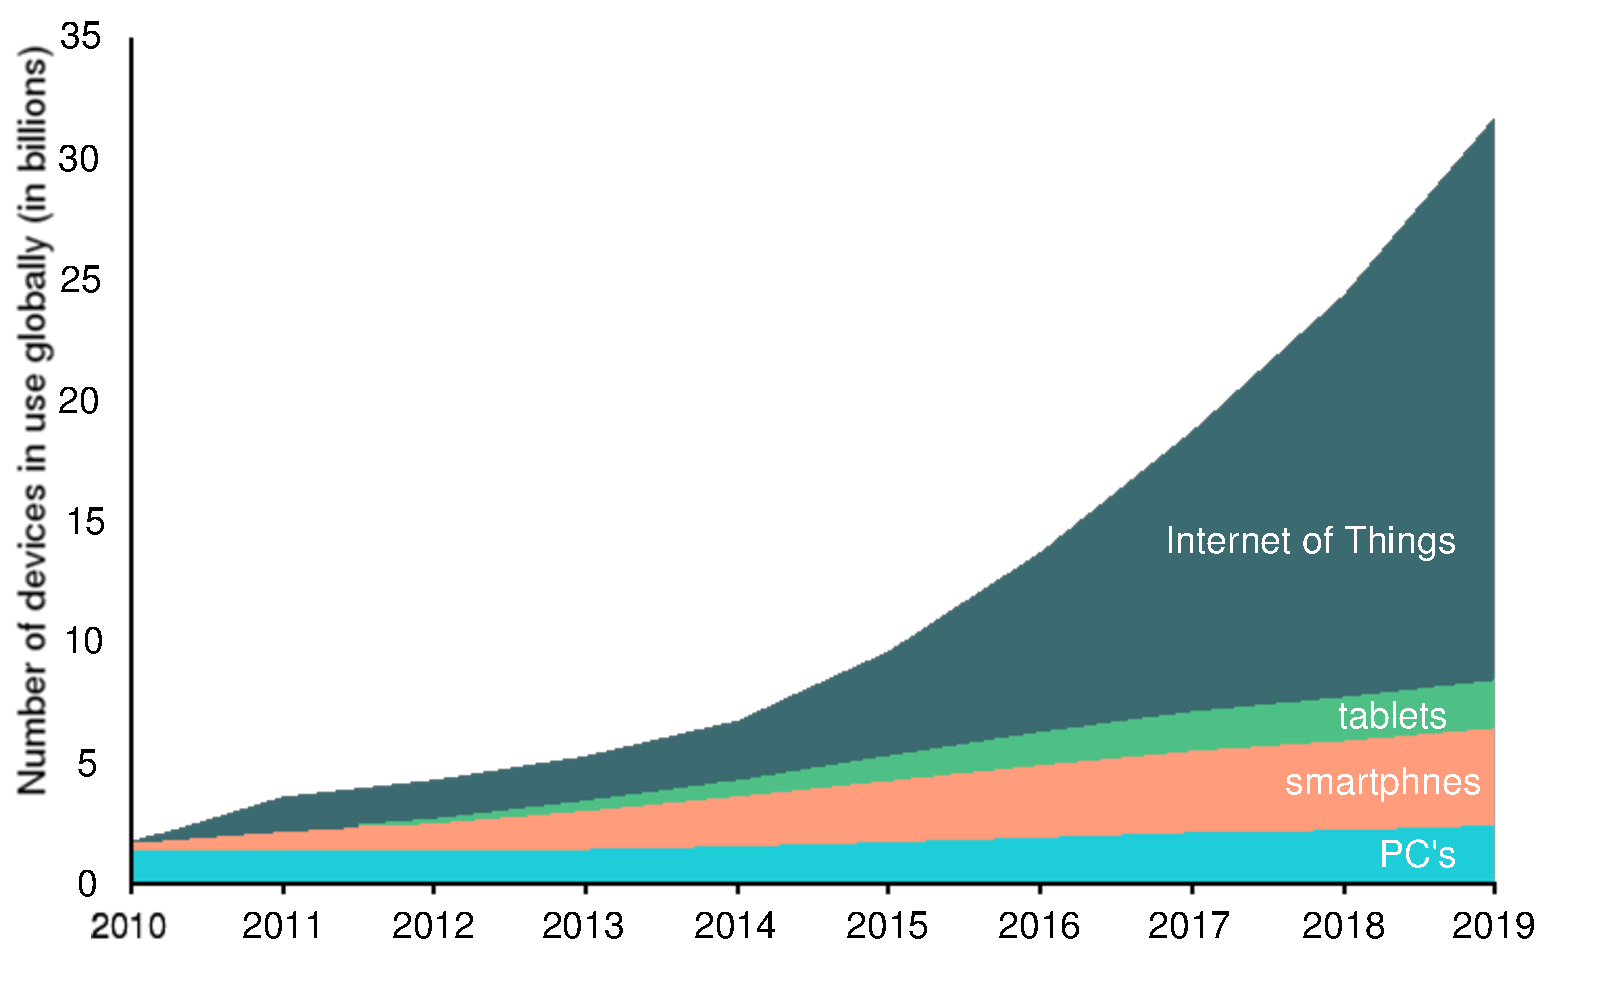
\includegraphics[width=10cm]{iot_devices}
\caption{Numero di dispositivi per anno}
\end{figure}

Questa rapida crescita ha portato alla ricerca è sviluppo di nuove soluzioni 
tecnologiche per supportare il carico di dispositivi simultaneamente connessi 
alla rete, senza avere un degrado evidente delle performance.
Per non alterare il \emph{QoS} Quality of Service della rete ed garantire costi
non elevati tecnologie come \emph{LPWAN} sono state ideate. I punti chiave per
garantire tutto ciò sono
\begin{itemize}
\item \textbf{Scalabilità}: Dato l'elevato numero di devices connessi, scenari
urbani ed industriali, la network tecnologi alla base dovrà essere estremamente
adattabile, in maniera dinamica, al carico di dispositivi connessi.
\item \textbf{Costo unitario}: Il costo del singolo modulo, dovrà essere basso
per garantire la più ampia fetta di mercato.
\item \textbf{Durata della batteria}: La maggior parte dei dispositivi sarà
alimentata tramite batteria, e la durata media e stimata di anni. 
\item \textbf{Costo computazionale}: La modulazione alla base di queste nuove
tipologie di rete, dovrà essere concepita in modo da non avere un costo
computazionale elevato.
\item \textbf{Distanza}: Un altro punto fondamentale è la possibilità di avere
comunicazioni a lunga distanza.
\end{itemize}

La rete di tipo \emph{LPWAN} è in grado di supportare tutti questi aspetti, le
principali tecnologie che già supportano questo tipo di rete son SigFox\tm,
LoRaWAN\tm, NB-IoT\tm e Weightless\tm. 

\begin{figure}[h]
\centering 
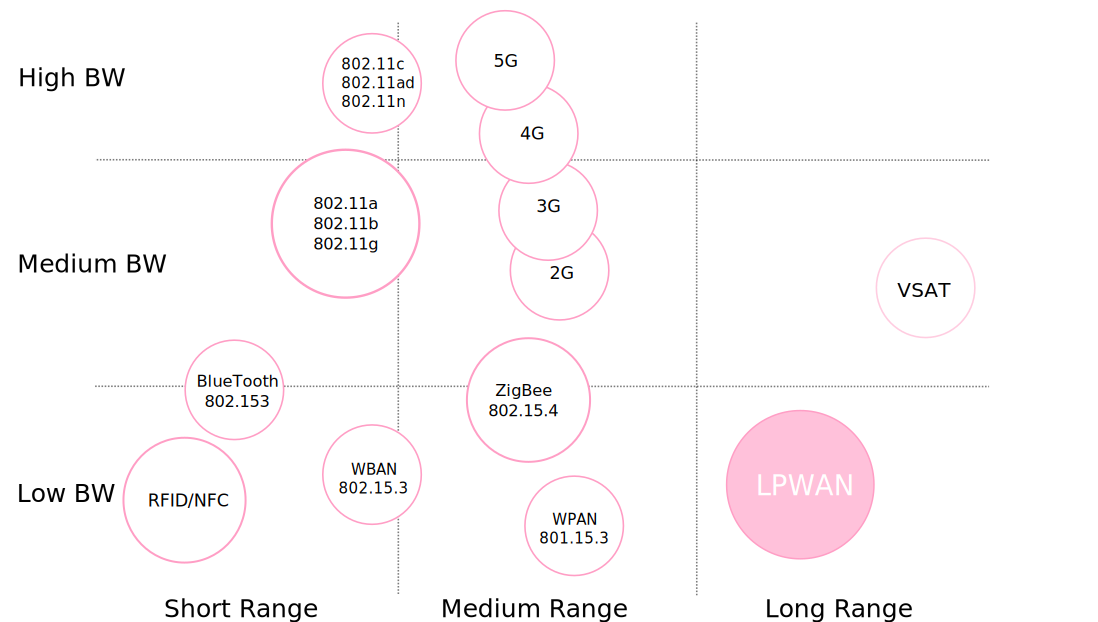
\includegraphics[width=15cm]{network_comp}
\caption{Comparazione tipologia di reti}
\end{figure}

Con questa tesi si è voluto studiare i casi applicativi della tecnologia Lora\tm
nel abito della agricoltura di precisione, utilizzando il framework open-source
Kura\tm messo a disposizione da Eurotech\tm, andando a creare un applicativo
OSGI\reg installabile nel framework. 


\mainmatter

\chapter{IoT}
L'Internet delle cose (Internet of Things, IoT) è un paradigma riferito
all’estensione di internet al mondo degli oggetti. Nel 1999 il ricercatore
britannico Kevin Ashton, durante una presentazione, teorizzò  per primo un mondo
nel quale oggetti ,dotati di sensori, interagiscono utilizzando la rete.  La
continua evoluzione delle tecnologie wireless e satellitari ha permesso
l'ideazione di oggetti sempre più connessi, in grado di generare una grande mole
di informazioni e dati. Oltre ai computer,smartphone e tablet, sempre più
oggetti di uso quotidiano dispongono di una connessione ad internet. Smartwatch
e smart band , lampadine e prese elettriche "intelligenti" ,  sono già da tempo
reperibili nel mercato\bx{,} con un prezzo accessibile alla stragrande maggioranza dei
consumatori.  Data la bassa
complessità del hardware ,implementato in questi devices, necessitano di
appoggiarsi ad un server esterno per l'elaborazione dei dati.  Sfruttando la
connessione ad internet, gli oggetti riescono ad instaurare uno scambio di dati
bidirezionale tra loro ed il server. Il dispositivo, infatti,  dopo aver
convertito la grandezza fisica di suo interesse in un dato comprensibile al
server, invia l'informazione \bx{a quest'ultimo}, il quale, dopo un'elaborazione della
stessa, formulerà dei comandi di risposta all'oggetto.
\\
\begin{figure}[h]
        \centering 
                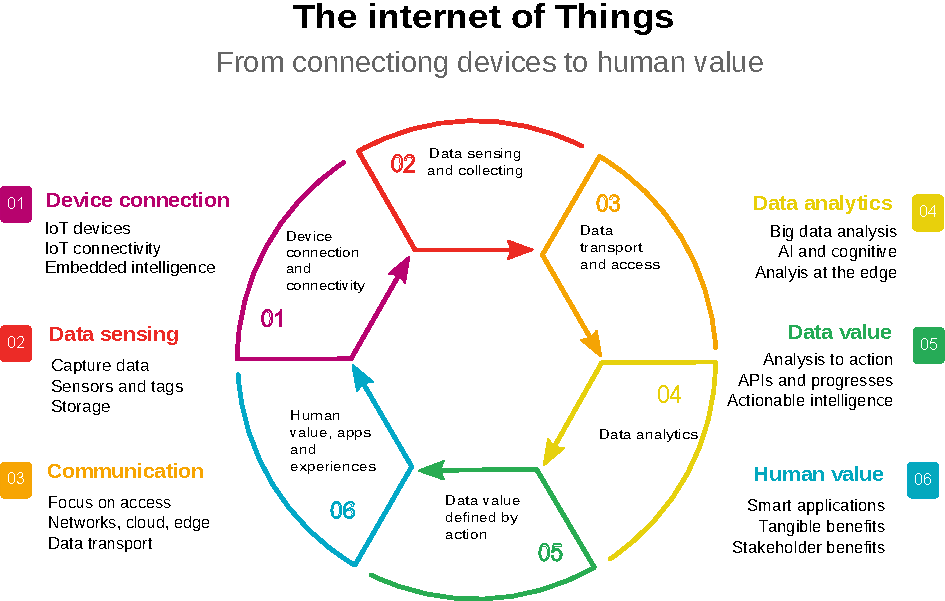
\includegraphics[width=16cm]{IoT-c1}
        \caption{Catena del valore dell'IoT}
        \label{fig:IoT_chain}
\end{figure}
I dati sono la materia prima del mondo dell'IoT, sono \bx{loro} che giocano il ruolo
principale sulla catena del valore (value chain), figura \ref{fig:IoT_chain},
dando una svolta importante ,dal
punto di vista economico, a nuovi settori quali il \emph{data mining} e la
\emph{business analysis}.
Attraverso lo studio delle informazioni presenti ,si potrà  aumentare l’efficienza di un
servizio oppure  migliorare la esperienza d'uso di una applicazione.
Muovendoci verso un modo sempre più connesso, nove problematiche riguardanti la
privacy e la sicurezza emergo.  Molto spesso, per tagliare i costi di produzione e
di sviluppo di questi gadget tecnologici, le aziende tendo a ridurre gli
investimenti nell'R\&D (Ricerca e Sviluppo), andando a produrre dispositivi con
un software non aggiornato o con componenti hardware di bassa qualità. Inoltre
, il ciclo vitale di un prodotto, non sarà più determinato solo dalla
rottura o dal mal funzionamento del dispositivo stesso ma, verrà ridotto dalla
impossibilità di un aggiornamento del firmware.
Le falle di sicurezza presenti nel software , ed il sempre più alto numero di
attacchi hacker, rappresentano un grave  pericolo per la sicurezza e la privacy del utente
finale.
È necessario quindi trovare un accordo, tra case produttrici e
consumatori ,al fine di garantire una \bx{life span minima}, di alcuni anni, per quanto
riguarda gli aggiornamenti. Riducendo così quello che più comunemente
viene chiamato il fenomeno della obsolescenza programmata. 
\section{Big Data}
Oltre all'innumerevole quantità di dati che verrà prodotta da questi milioni di
devices intelligenti, noi stessi,  navigando il web, ne produciamo una grande
quantità. Nel 2013\bx{,} si è stimato che ogni secondo nel web venivano generati una
quantità di dati pari a 28875GB . Con il  termine Big Data, si vuole
rappresentare l'insieme di tutti i dati eterogenei\bx{,} che ogni giorno vengono
prodotti e scambiati nella rete.
Con il progredire della tecnologia il dataset (aggregazione di dati) a
disposizione delle aziende è in continuo aumento.
Secondo un articolo pubblicato da Verizon, si stima che il 92\% delle aziende
usa meno del 25\% dei dati raccolti e che solo la metà  di esse prevede di
riuscire a fare fruttare una percentuale maggiore di quella attuale,nei prossimi due anni
\cite{Verizon}.  Con “Data mining” o "Data analytics"  si identificano tutte le
tecniche e le metodologie finalizzate all’estrazione di sapere e conoscenza
partendo da una vasta mole di dati.
L’enorme disponibilità, di ogni sorta di informazione, è una prospettiva che 
apre innumerevoli scenari di ricerca; ad esempio, predire con largo anticipo i 
trend del mercato, permetterebbe ,ad una azienda, di investire in maniera più
efficace le proprie risorse, andando a creare un maggiore profitto.


\section{La diffusione dell'Internet delle cose}
Nel 2008\bx{,} il numero di oggetti quali personal-computer, server, telefoni cellulari,
connessi ad internet, ha superato il numero di persone presenti nell'intero
pianeta. Il continuo sviluppo tecnologico, la sempre maggior facilità d'uso e
l'abbattimento dei costi, ha reso disponibile, al mondo consumer, tecnologie che
fino a poco tempo fa erano destinate ad un uso aziendale ed universitario. 
Con l'avvento dell'IoT, si prevede una crescita esponenziale di devices connessi
ad Internet;  secondo  una stima da parte di Gartner, il numero di smart
device presenti nell'anno 2020, sarà superiore a 20 miliardi \cite{gartner2016}.
Per fronteggiare una crescita così esponenziale, è d'obbligo cercare soluzioni
in grado di prevenire il congestionamento della rete. 
\\
\begin{table}[h]
        \centering
        \begin{tabular}{l|c|c|c|c}
                \textbf{Categoria}  & 2016 & 2017 & 2018 & 2019 \\
                \hline
                \emph{Consumer}  & 3963 & 5244,3 & 7063,3 & 12863 \\
                \emph{Business}  & 1418 & 2135.4 & 4152,7 & 6171  \\
                \emph{Totale }   & 6381 & 8380   & 11196  & 20415 \\
        \end{tabular}
        \caption{Stima di dispositivi IoT (Milioni di unità)
        Gartner\cite{gartner2016}}
\end{table}
\\
\begin{figure}[h]
        \centering 
                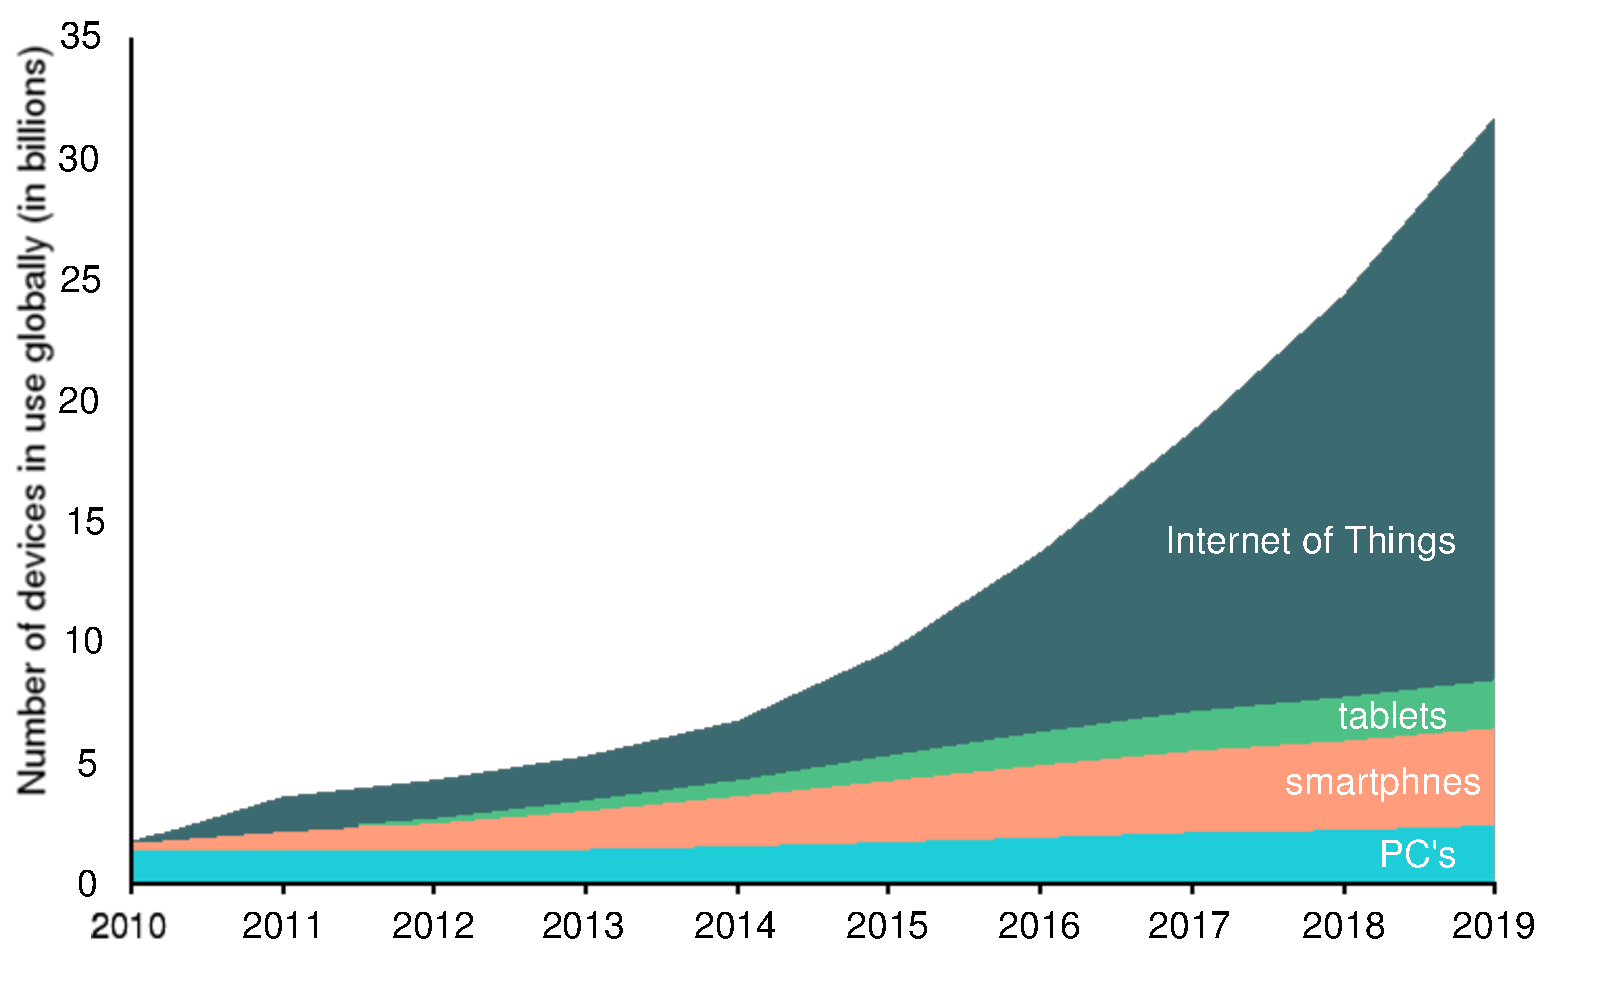
\includegraphics[width=10cm]{iot_devices}
        \caption{Numero di dispositivi per anno}
\end{figure}

\section{Business}
Considerando le statistiche precedenti, è comprensibile che l'IoT sia un
mercato che agisce in maniera trasversale su tutti i settori.  Se l'utilizzo di
sensori in ambiti quali la domotica e l'automotive è da tempo largamente
impiegato, grazie all'abbattimento del costi del
singolo  dispositivo e la facile implementazione di queste nuove tecnologie,  nuovi
mercati e nuove possibilità di investimento sono nate. Prendiamo come esempio
l'agricoltura di precisione, che grazie a sensori in grado di rilevare dati
riguardanti l'umidità del suolo, l'indice di piovosità oppure l'umidità fogliare,
permette all'agricoltore di  capire quando è il momento di intervenire per il
trattamento delle colture. In questo modo è possibile dispiegare le risorse in
maniera più efficace, andando ad agire solo nelle culture danneggiate.Sempre
secondo quanto stimato da Gartner, ci si aspetta che entro il 2020, 
la cifra investita nell'idustria del IoT,
sarà pari a circa \$3,000,000 milioni di dollari con un investimento annuo di
circa \$500,000 milioni di dollari. È utile osservare, che la più grande fetta e quella
riservata al mercato consumer dove smart TV, set-top box e smart cars saranno i prodotti
maggiormente richiesti.
\cite{gartner2016}. 



\section{La tecnologia alla base dell'IoT} 
Nell'industria il concetto di M2M (Machine to Machine) non è un concetto nuovo,
già Kevin Ashton, durante la presentazione in cui introdusse il termine IoT,
comprese le potenzialità della tecnologia RFID applicate alla supply chain. Dal
1999 ad oggi molte cose sono cambiate, ma molte domande non hanno ancora trovato
una risposta. Come accadde agli albori di Internet, quello che manca al modo
dell'IoT è una standardizzazione dei protocolli e del linguaggio con cui questi
oggetti devono comunicare. Astraendoci dal problema e portandoci ad una visione
di più alto livello problema, è possibile individuare in questo paradigma
tre livelli.
\begin{figure}[h]
        \centering 
                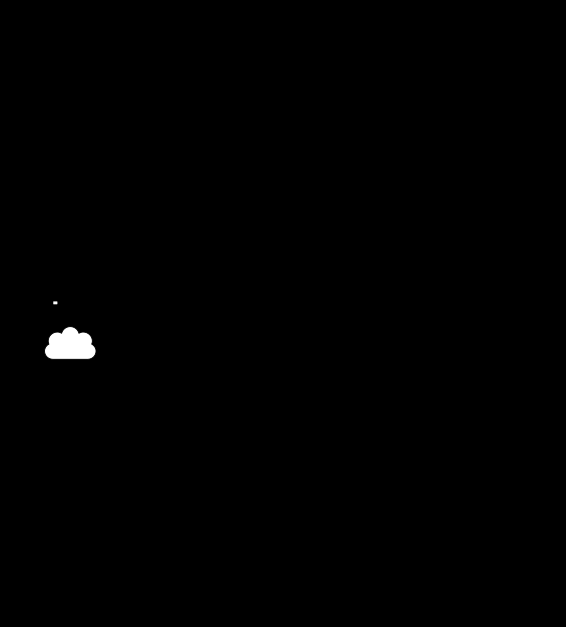
\includegraphics[width=10cm]{three-layer}
        \caption{Layer del IoT}
\end{figure}
\begin{itemize}
\item \textbf{Device layer} o sensor layer, è il layer più basso. Esso raggruppa
tutti i gli oggetti "smart". Questo layer è quello che mette in comunicazione il
mondo reale con gli atri layer superiori. A loro spetta lo scopo di convertire
una misura fisica in un segnale interpretabile da altri calcolatori.
La maggior parte di questi sensori, utilizzerà una connessione Bluetooth,
ZigBee, Wifi o una si baserà su una rete LPWAN per comunicare il dato al layer
superiore.
\item \textbf{Network layer} o mediation layer raggruppa l'intera infrastruttura
di rete e gateway che ricevono i dati da i vari sensori. Questo layer è
semplicemente un layer di mediazione dove l'informazione (dato) non viene altera
ma semplicemente trasmesso all'Application layer.
\item \textbf{Application layer} è il layer nel quale l'informazione viene
immagazzinata ed elaborata. Questo layer è il più importante, e qui dove il dato
viene trasformato da una semplice misurazione fisica ad una possibile revenue
per l'azienda che lo gestisce.%\improvement{Riscrivere}
\end{itemize}
Già molte sono le aziende che si sono mosse per cercare di imporsi in questo
mercato fiorente. Data la vastità dei campi di applicazione, non è semplice
prevedere quale standard predominerà sugli altri.
Aziende del calibro di Samsung con la
piattaforma \href{https://www.artik.io}{artik}  , Zigbee con
\href{https://www.speakdotdot.com/dotdot/}{DotDot} e Google con
\href{https://developers.nest.com/weave/}{Weave}, hanno già proposto delle
possibili soluzioni per il "linguaggio" universale utilizzabile dai vari
dispositivi. Un dibattito ancora più acceso  riguarda i protocolli e la topologia di
rete da utilizzare. Dovendo superare i limiti delle tecnologie attuali, sono
molteplici le problematiche che devono essere affrontate per poter offrire una
architettura adattabile ai vari use-case dell'IoT.
Con questa tesi si cercherà di  approfondire lo stato dell'arte del network layer
andando a esporre le principali tecnologie ad oggi presenti sul mercato. In
particolare verrà posta l'attenzione sulla tecnologia LoRaWAN e una sua possibile
implementazione all'interno del framework Kura/ESF sviluppato da Eurotech.




%\section{IoT}
Sempre più spesso si parla di Internet delle cose, o IOT, con questo termine si 
intende un evoluzione delle applicazioni legate al settore mobile, al settore
della home automation e al settore embedded. 
In questo scenario ogni oggetto il
quale contiene un sensore sarà connesso ad Internet. Avvalendosi di questa
connessione , i vari dati raccolti potranno essere inviati nel cloud, dove
verranno elaborati e resi disponibili alle varie applicazioni. 
Per fare in modo che questo update avvenga, è necessario riuscire a creare una
rete di devices ,correlati nelle loro funzionalità, i quali riescano a
\emph{parlare un linguaggio comune}. \improvement{Scrivi qualcosa di decente
qui}
Il punto principale di questo
upgrade sta nel riuscire a creare una rete di devices connessi ad internet. Per
supportare e utilizzare una potenza di calcolo maggiore andando a combinare
tecniche di data analytics per estrarre le informazioni più significative. 

In
questa visione, milioni di devices saranno connessi a Internet e molto presto
milioni di milioni di devices. 

Il mercato di questi \emph{smart devices } è
in rapida crescita con una stima di 8,3 miliardi di dispositivi connessi nel
anno 2017, e di circa 20 miliardi per l'anno 2020 \cite{gartner2016}. Andando ad
creare un impatto economico compreso tra i 2.7 e i 14 trilioni di dollari. I
mercati principali saranno quelli del healt care con un introito compreso tra i
$1.1$ e i $2.5$ trilioni di dollari e il settore industriale con $2.3$ a $11.6$
trilioni di dollari.

\begin{figure}[h]
\centering 
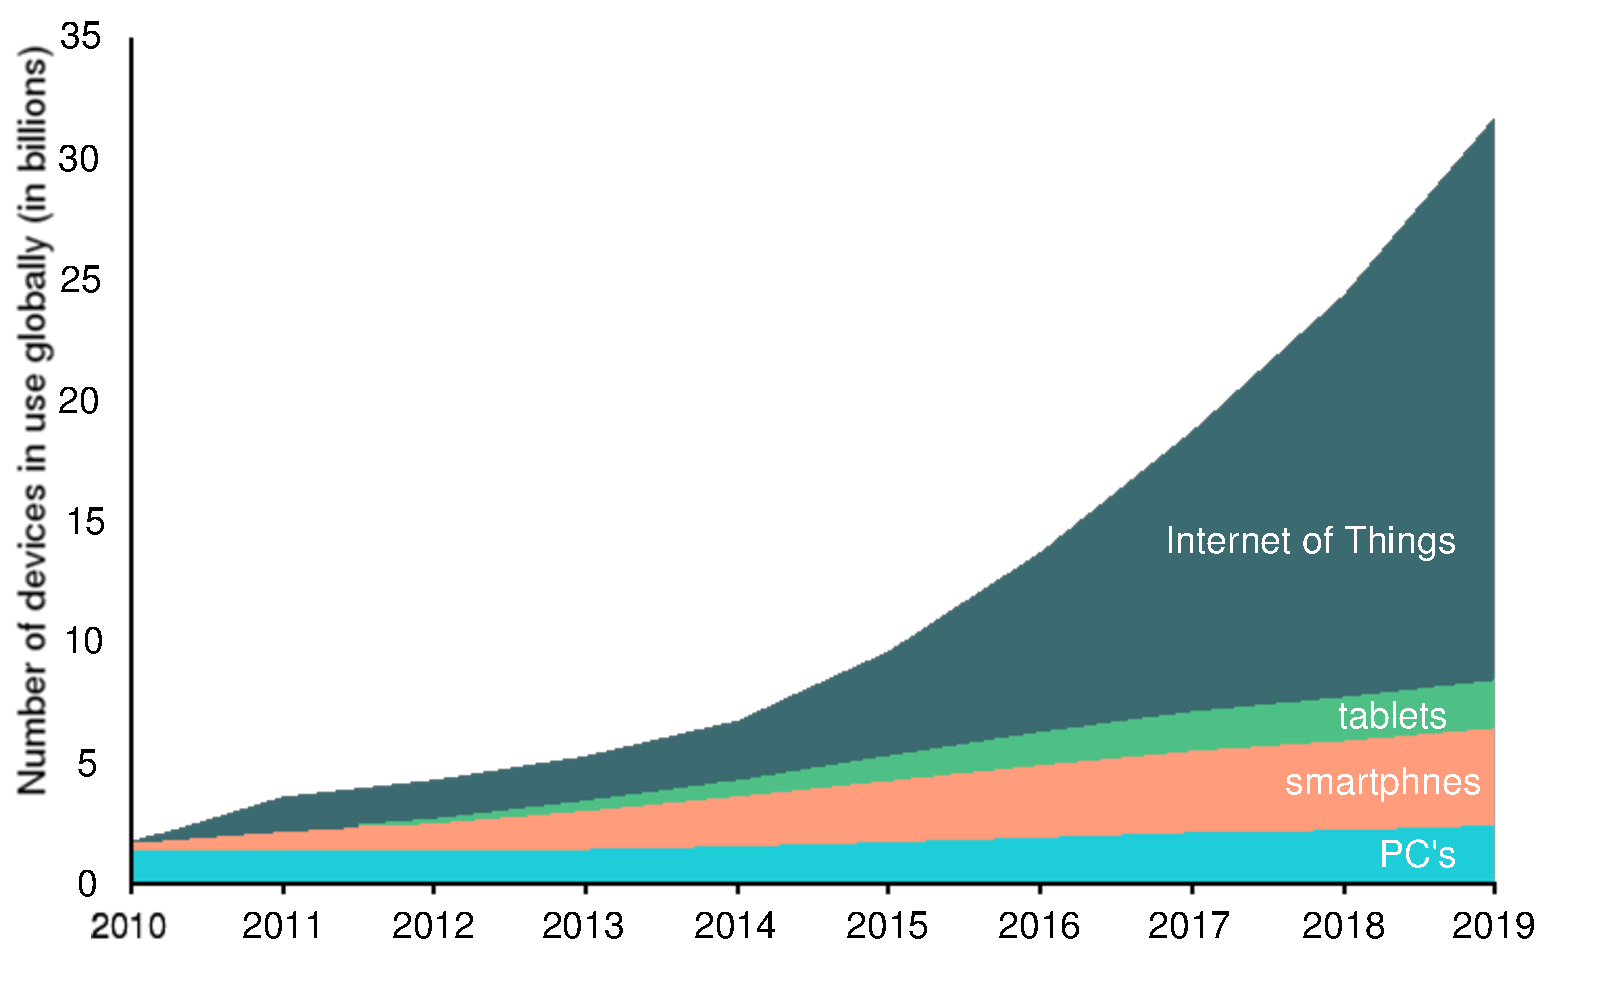
\includegraphics[width=10cm]{iot_devices}
\caption{Numero di dispositivi per anno}
\end{figure}

Questa rapida crescita ha portato alla ricerca è sviluppo di nuove soluzioni 
tecnologiche per supportare il carico di dispositivi simultaneamente connessi 
alla rete, senza avere un degrado evidente delle performance.
Per non alterare il \emph{QoS} Quality of Service della rete , hardware e
software dovranno essere rivisti insieme alla topologia di rete utilizzata. I
principali punti chiave sono

\begin{itemize}
\item \textbf{Scalabilità}: Dato l'elevato numero di devices connessi, scenari
urbani ed industriali, la network tecnologi alla base dovrà essere estremamente
adattabile, in maniera dinamica, al carico di dispositivi connessi.
\item \textbf{Costo unitario}: Il costo del singolo modulo, dovrà essere basso
per garantire la più ampia fetta di mercato.
\item \textbf{Durata della batteria}: La maggior parte dei dispositivi sarà
alimentata tramite batteria, e la durata media e stimata di anni. 
\item \textbf{Costo computazionale}: La modulazione alla base di queste nuove
tipologie di rete, dovrà essere concepita in modo da non avere un costo
computazionale elevato.
\item \textbf{Distanza}: Un altro punto fondamentale è la possibilità di avere
comunicazioni a lunga distanza.
\item \textbf{Sicurezza}: Ogni devices dovrà essere difficilmente penetrabile da
attacchi esterni.
\item \textbf{Menagment}: I vari dispositivi dovranno essere facilmente
controllabili da remoto.
\item \textbf{Fail-safe}: Il non funzionamento di devices non dovrà
compromettere l'intera infrastruttura a lui connessa. 
\end{itemize}

Vari tipi di architetture di rete sono stati proposti per realizzare questa
nuova infrastruttura. Per quanto le varie proposte si basano su tecnologie
differenti, è possibile individuare tre layer comuni 
\begin{itemize}
\item \textbf{Device layer} formato da tutti i dispositivi che collezionano dati
e sono connessi alla rete.
\item \textbf{Network layer} La struttura della rete, la quale permette di
connettere i vari devices in modo che possano scambiare i dati tra di loro o
inviarli ad un data-center.
\item \textbf{Application layer} il quale interpreta e utilizza i dati ricevuti.
\end{itemize}

Attualmente sono diversi i concorrenti che provano ad affermarsi nel settore
del IoT proponendo soluzioni diverse. Nei seguenti capitoli ci sarà un analisi
generale delle varie topologie proposte, in particolare verrà analizzata la
tecnologia Lora ed il protocolla LoraWAN.


\chapter{LPWAN}
Data la grande varietà dei possibili scenari applicativi dell'IoT , trovare uno standard
capace di adattarsi, in modo dinamico, ad ognuno di essi, non è un compito
facile. Le tecnologie wireless tradizionali, non sono in grado di soddisfare
la dinamicità  di questo paradigma.
Già diverse soluzioni sono nate per cercare di fronteggiare questi
problemi, optando per metodi risolutivi  anche molto distanti l'uno dall'altro.
Con questo capitolo si approfondiranno le problematiche, che i nuovi standard, riguardanti il
network layer, dovranno essere in grado di risolvere.
\section{Alla base delle reti LPWAN}  
Le tecnologie wireless com ZigBee, WiFi, non sono ideate per connettere devices
alimentati a batteria distribuiti in una vasta area geografica.
Il range di queste tecnologie è limitato a poche centinaia di metri al massimo.
Tutto ciò implica che i devices, non possono essere implementati in tutti gli
ambienti, ma solo in uno spazio ristretto alla portata del segnale del gateway.
Quindi scenari quali la sicurezza sanitaria, agricoltura di precisione, logistica non
permettono l'utilizzo di questa tecnologia.
La grande copertura offerta dalle tecnologia cellulare è la ragione per la quale
è ad oggi la tecnologia più utilizzata nelle comunicazioni M2M.
Tuttavia, il continuo progresso tecnologico, sta portando l'abbandono della rete
GSM da parte degli operatori telefonici, per poter riutilizzare le bande da essa
occupata con tecnologie più innovative. In generale, la tecnologia cellulare non
garantisce una durata della batteria molto prolungata ed inoltre il costo
complessivo dei moduli cellulari è molto elevato, data la complessità delle 
forme d'onda .

Dovendo ingegnerizzare il network layer, è importante capire quali sono le
principali problematiche che le tecnologie attuali non sono in grado di colmare.

\begin{itemize}
\item \textit{Indirizzabilità}: a causa dell’elevato numero di oggetti che entrano in
gioco in IoT, la capacità di indirizzamento di IPv4 non è più suffi-
ciente. IPv4 usa 32 bit per gli indirizzi, quindi ce ne possono essere
massimo $2^{32}$ diversi. Il passaggio a IPv6 risolverà il problema, in quanto si passerà da
32 bit a 128 bit per gli indirizzi. 
\item \textit{Scalabilità}: Dato l'elevato numero di devices previsti nei scenari
urbani ed industriali, la network technology alla base della rete dovrà essere 
adattabile, in modo dinamico, al carico di dispositivi connessi.
\item \textit{"Arrive and operate”}: dispositivi mobili eventualmente aggiunti do-
po la formazione iniziale del sistema, non devono aver bisogno di
configurazione, ma devono essere in grado di stabilire connessioni
autonomamente con gli altri oggetti già presenti.
\item \textit{Costo unitario}: Il costo del end device, dovrà essere conveniente
per garantire la più ampia fetta di mercato.
\item \textit{Fonti di energia}: 
Gli oggetti nella maggior parte dei casi sono mobili, quindi non han-
no sempre la possibilità di essere collegati a una fonte di energia. Le
batterie inoltre sono pesanti e grandi.È necessario quindi andare a ridurre la quantità 
di energia richiesta dagli oggetti, andando ad aumentare il tempo di deep-sleep
.
\item \textit{Interoperabilità}: gli oggetti sono di natura diversa (per esempio
possono avere requisiti di larghezza di banda diversi, o hardware diverso).
Questo implica la necessità di standard, in modo che oggetti di tipo
diverso possano comunicare tra loro
\item \textit{Costo computazionale}: La modulazione, alla base di queste nuove
tipologie di rete, dovrà essere concepita in modo da non richiedere un costo
computazionale elevato .
\item \textit{Raggio d'azione}: La necessità di utilizzare questi devices in ambienti
difficili o rurali, rende necessario l'utilizzo di tecnologie wireless con un
raggio di azione dell'ordine di una decina di chilometri.
\item \textit{Sicurezza}: Lo scambio dei dati dovrà avvenire in maniera sicura,
implementando algoritmi di cifratura dei dati o procedure di handshaking.
\item \textit{Tolleranza ai guasti}: Il mal funzionamento  o il guasto di un
nodo della rete,  non dovrà compromettere il funzionamento dell'intera rete a lui connessa. 
\end{itemize}

\section{LPWAN}
Per colmare il gap tra tecnologie esistenti e la
necessita di connettere milioni di devices diversi, sono nate le  LPWAN
\emph{Low power wide area network}.
Le reti LPWAN rappresentano un modello  di comunicazione
innovativo, che integra le tecnologie cellulari tradizionali e quelle a corto
raggio per affrontare diverse esigenze delle applicazioni IoT. 
Le reti LPWA, andando a sacrificare il massimo throughput dei devices, ne sono in
grado di gestire un gran numero contemporaneamente, cosa che con le tecnologie
wireless tradizionali non è possibile realizzare.

\begin{figure}[ht]
    \centering 
        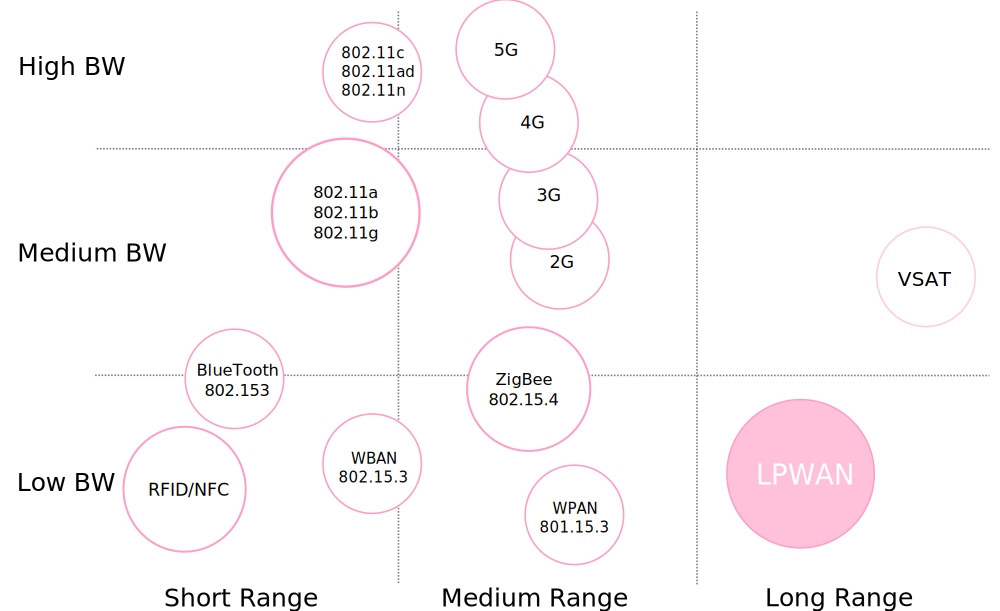
\includegraphics[width=12cm]{network-com}
    \caption{Comparazione tipologia di reti}
\end{figure}

In questo contesto, i maggiori competitor sono  NB-IoT, EC-GSM-IoT
LTE-M, SigFox e Lora. Le prime tre  sono una evoluzione delle precedenti reti
cellulari 2G,3G e 4G. Operando sulle bande di frequenza licenziate, e necessario
che ognuna di queste tecnologie sia approvata dalla 3GPP ( 3rd Generation
Partnership Project), la quale si occupa della standardizzazione dei sistemi di
telecomunicazione a livello internazionale.
All'opposto, Sigfox e Lora sono due tecnologie che operano nelle frequenze ISM
(Industrial, Scientific and Medical). Le frequenze ISM sono uno spettro radio
riservato alle applicazioni di radiocomunicazione non commerciali.

\begin{figure}[ht]
    \centering 
        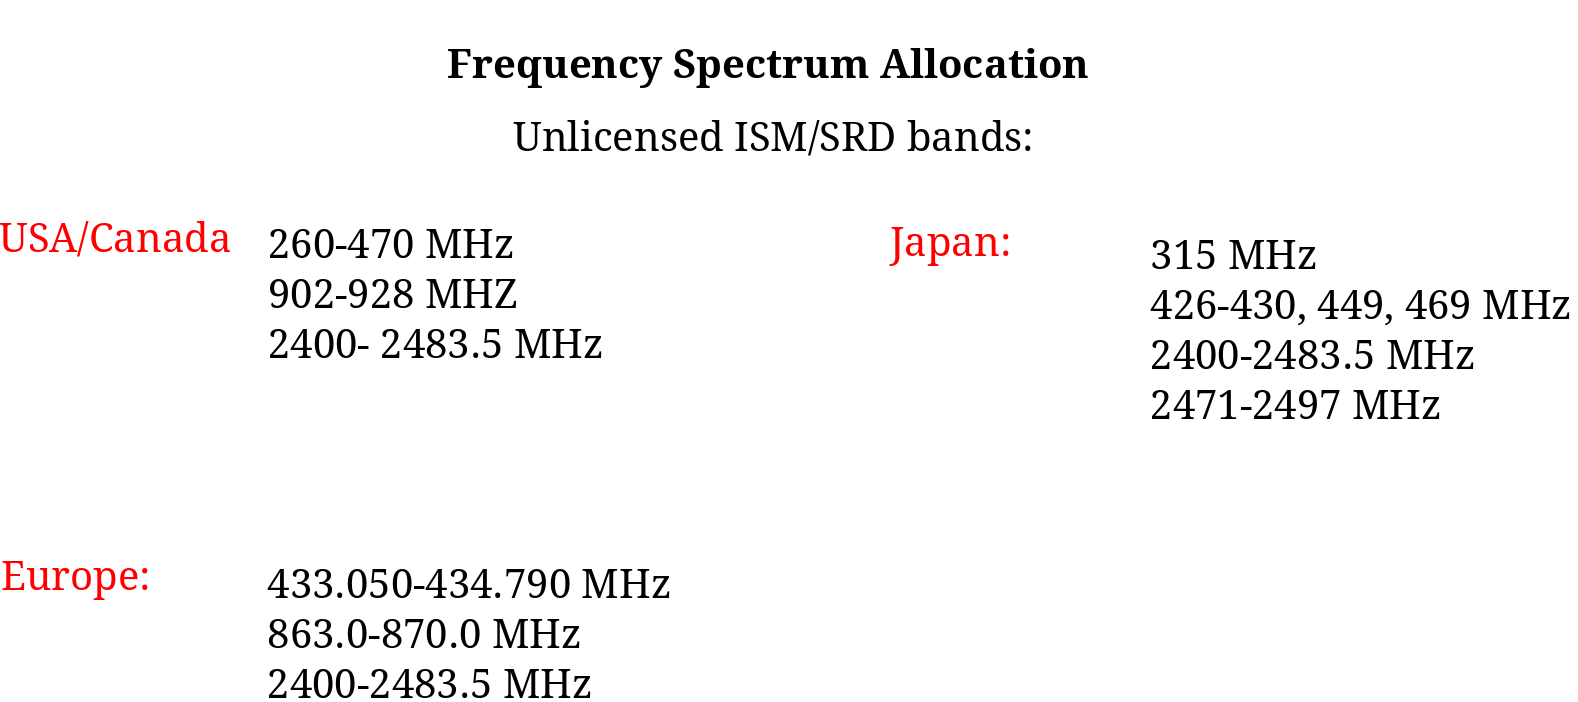
\includegraphics[width=10cm]{Orignal/freq}
    \caption{Comparazione tipologia di reti}
\end{figure}

In particolare entrambe le tecnologie operano  nella banda degli 868 [MHz]
la quale permette una potenza del segnale inviato massima pari a 14 [dbm] ed un
duty cycle inferiore al 1\%.
 
\section{NB-IoT}
Narrowband IoT (NB-IoT) o LTE Cat NB1 è uno standard certificato nella release 13 del 3GPP, la
quale riutilizza le infrastrutture già presenti, quali 2G, 3G, 4G per la rapida
realizzazione di una rete LPWA per l'IoT.
Focalizzandosi sulla durata della batteria, i moduli NB-IoT risultano avere un
costo all'unità minore del 75\% rispetto ad un normale modulo LTE.
Basato sulle frequenze licenziate, NB-IoT è in grado di
offrire tre diversi scenari di sviluppo \cite{NB-white_paper}
\begin{itemize}
\item \emph{standalone}, utilizzando qualsiasi spettro disponibile dell'
operatore.
\item \emph{guard band}, utilizzando lo spettro libero presente tra due bande
radio, per prevenire interferenze.
\item \emph{in band}, utilizzando lo stesso spettro della banda LTE.
\end{itemize}
\begin{figure}[ht]
    \centering 
        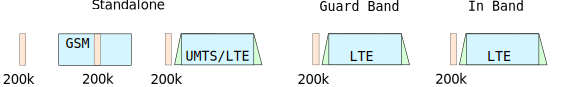
\includegraphics[width=12cm]{nb-iot}
    \caption{Modalità di funzionamento NB-IoT}
\end{figure}
L'obbiettivo che NB-IoT si prefigge è quello di mettere a disposizione una
tecnologia con una elevata copertura ed un basso data-rate. La possibilità di
riutilizzare strutture già esistenti, ed il basso costo per device , rendo
NB-IoT, una delle tecnologie che sta riscuotendo maggiore successo nel abito IoT.



\section{LTE-M}
Dalla realise 8 del 3GPP, diverse nuove tipologie di rete LTE sono disponibili.
La categoria che offre le migliori performance batteria/data-rate è la categoria
LTE Cat-M1 o LTE-M.
Questa categoria ,a differenza del NB-IoT, rispecchia lo standard LTE in pieno, 
implementando  la Frequency Division Multiplexing
(FDM) e Time Division Multiplexing (TDM). Risultando adatta per applicazioni
nelle quali è necessario l'invio di dati audio o video oppure per comunicazioni a
bassa latenza . Il data-rate raggiungibile è pari a 5Mbps in
uplink e 10 [Mbps] in downlink .  Questo tipo di connessione sarà utile
per tutte quelle applicazioni in cui è richiesta una elevata sicurezza del dato
da trasmettere, come ad esempio applicazioni di video-sorveglianza o automotive
.Questa tecnologia ,già disponibile negli Stati Uniti tramite la rete Verizon, è
in fase di roll out per molti operatori europei.

\section{EC-GSM-IoT}
EC-GSM-IoT si basa su funzionalità aggiuntive a partire da EGPRS che consentono
ad una rete GSM/EDGE di essere predisposta per fornire servizi IoT. Lo standard
è stato pensato in particolare per quei Paesi, come quelli in via di sviluppo,
dove una rete LTE non è ancora disponibile. L’occupazione spettrale di ogni
canale corrisponde a  200 kHz.  Tuttavia, al fine di dispiegare EC-GSM-IoT, si
richiede una banda utile di 2.4 MHz per permettere il frequency hopping , che,
con l’aggiunta di 2 canali di guardia di 200 kHz ciascuno agli estremi della
banda, porta l’occupazione di banda complessiva a 2.8 MHz.  La
potenza di trasmissione del Il data rate di picco raggiungibile sia in DL sia in
UL è di 491 kbps, mentre il valore mediato nominale è di 98 kbps sia in DL sia
in UL. Al fine di soddisfare i requisiti di capacità (più di 50.000 terminali in
ogni singolo settore di una cella trisettoriale). 

La figura \ref{tab:IoT_cell_comp} riassume in breve le varie caratteristiche
delle reti cellulari facenti parte della categoria LPWA
\begin{table}[h]
    \centering 
                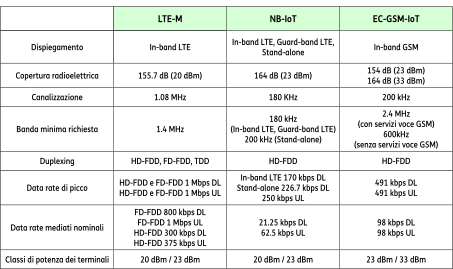
\includegraphics[width=12cm]{tim_iot}
    \caption{Comparazione reti cellulari per l'IoT}
    \label{tab:IoT_cell_comp} 
\end{table}



\section{Sigfox}
SigFox, azienda francese, sta sviluppando in partnership con altri operatori di
rete una soluzione LPWAN basata sulla sua tecnologia. Sigfox punta alla
costruzione di una rete mondiale proprietaria basata su frequenze ISM.
Correntemente SigFox è presente in Francia, Belgio, Olanda e Portogallo come
illustrato nella figura \ref{fig:Sig_covereg}.
\begin{figure}[h]
    \centering 
                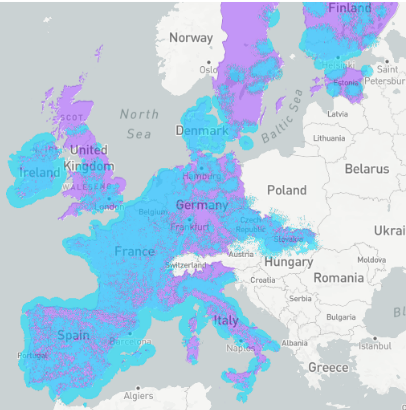
\includegraphics[width=12cm]{SigFox_covereg}
    \caption{Mappa copertura SigFox}
    \label{fig:Sig_covereg} 
\end{figure}

Gli end-devices comunicano con le varie base stations usando una modulazione (BPSK)
\emph{Binary Phase Shift Keying} con una banda di soli 100 [Hz]. 
Per via delle regolazioni vigenti nello spettro ISM, è per garantire una durata
della batteria pari ad una decina di anni, il numero massimo di messaggi
inviabili in un giorno è 140, con lunghezza del payload pari a 12 [byte] e un
throughput pari a 100 [bps]. SigFox si colloca come rete LPWAN con il minore
throughput, limitando il numero di use-case possibili. Inizialmente SigFox
supportava solo comunicazioni unidirezionali, successivamente, ha introdotto la
possibilità di avere una comunicazione bidirezionale, limitando il numero di
byte trasmissibili da gateway a devices a 4-8 bytes per giorno.

\section{LoRaWAN}
\emph{LoraWAN} è una tecnologia di modulazione wireless semi-proprietaria 
sviluppata da Semtech. Essa è composta da un layer fisico ,proprietario, che
prende il nome di \emph{Lora}\cite{LoRaCss101} , e una parte libera chiamata 
LoRaWAN\cite{LoRaWAN101} nella quale viene definito un protocollo di comunicazione, 
il quale usa LoRa come layer fisico. 
Basandosi su una tecnica di comunicazione a \emph{spread spectrum}, LoRa è in
grado di instaurare una comunicazione bidirezionale tra device e gateway.
I punti chiave dei questa tecnologia sono il grande raggio di copertura , il 
basso consumo energetico e la capacità di adattare in maniera dinamica il
data rate, il quale può variare dai 0.3 ai 50 [Kbps] a seconda dell'utilizzo. 
Come per SigFox, la tecnologia sviluppata da Semtech, si basa sulle bande ISM,
inoltre Essendo il protocollo LoRaWAN open source, si ha la possibilità di
creare delle reti pubbliche o private senza disporre di alcuna licenza, 
riducendo così il time to market di questa tecnologia.  
Progetti come \href{https://www.thethingsnetwork.org/}{The Things Network}
mirano a creare una rete LoRa ,pubblica è privata,  a livello globale.

\section{Osservazioni}
In questo mercato frammentato, non è semplice capire quale tecnologia sia adatta
a ricoprire una data applicazione. Essendo questi standard molto giovani, è
complicato comprendere le reali potenzialità di ognuna di queste soluzioni.
Quello che è possibile prevedere, sarà un incremento esponenziale di device che
stanno alla base della piramide in figura \ref{fig:pyramid}, devices i quali
potranno essere utilizzati in innumerevoli settori, non ancora esplorati dalle
tecnologie attuali, come per esempio i contatori della dell'acqua, applicazioni
per l'agricoltura di precisione e così via. 

\begin{figure}[ht]
    \centering 
                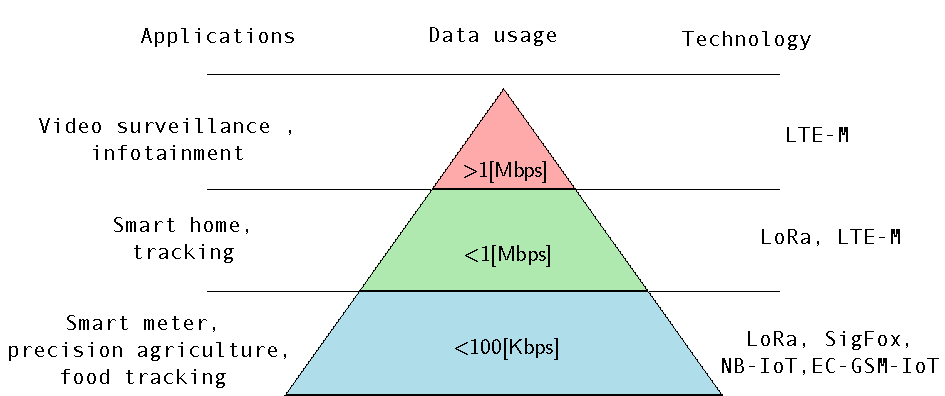
\includegraphics[width=12cm]{pyramid}
    \caption{Capacità delle reti LPWA}
    \label{fig:pyramid} 
\end{figure}

\pagebreak
Per le aziende, che si apprestano ad investire sul mondo dell'IoT, la scelta
della corretta tecnologia su cui andare a sviluppare i loro servizi non risulta
semplice, in quanto, fattori quali sicurezza, aggiornamenti software,
affidabilità devono essere ancora testati a pieno. Con la figura
\ref{fig:feature_comp} si vuole riassumere in breve i punti chiave delle
tecnologie appena trattate.

\begin{figure}[ht]
    \centering 
                \includegraphics[width=9cm]{Comparsion_no_line}
    \caption{Comparazione feature reti LPWAN}
    \label{fig:feature_comp} 
\end{figure}

Nel prossimo capitolo verrà analizzata in dettaglio la soluzione che Semtech
propone, approfondendo il layer fisico \emph{Lora} e la struttura del protocollo
LoRaWAN.

\section{LPWAN}
Il principale problema che si presenta nella ottica del IoT è avere una
infrastruttura di rete capace di gestire il traffico di milioni di dispositivi
contemporaneamente connessi.  Fino ad oggi la principale tecnologia wireless 
usata nelle comunicazioni M2M è stata la rete cellulare, la quale copre la quasi
totalità di tutte le aree geografiche.
La scelta della rete 2G, 3G, 4G è svantaggiosa poiché offre data-rate molto
maggiore rispetto a quello normalmente utilizzato in applicazioni IoT,
comportando l'uso di moduli sovradimensionati e andando ad aumentare di molto il
prezzo per unità. Inoltre l'elevato consumo energetico e il prezzo svantaggioso
degli abbonamenti offerti dagli operatori telefonici, ha portato alla ricerca di
nuovi standard. 
Per colmare il gap tra tecnologie esistenti e la necessita di connettere milioni
di devices diversi sono nate le   LPWAN \emph{Low power wide area network}.
Con questo termine, si identificano tutte quelle reti ideate appositamente per
l'IoT, le quali garantiscono una ampio raggio di azione, andando a sacrificare
il bit rate e la complessità dei moduli radio.

\begin{figure}[h]
        \centering 
                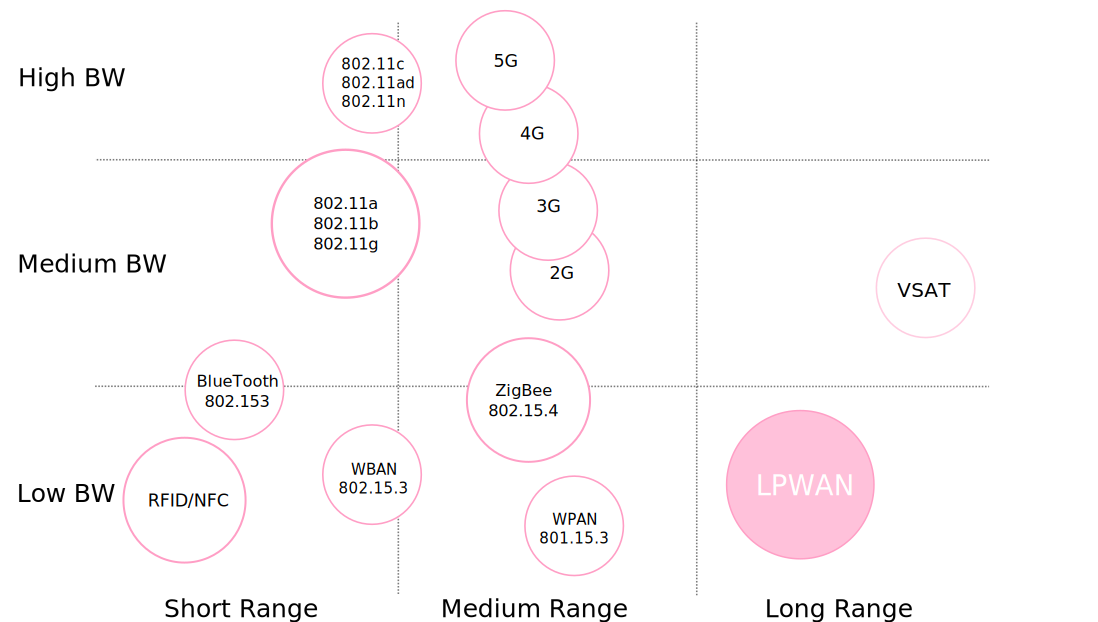
\includegraphics[width=16cm]{network_comp}
        \caption{Comparazione tipologia di reti}
\end{figure}

In questo contesto, i maggiori competitor sono Lora, Sigfox, NB-IoT e LTE-M.
Anche se ognuna di queste soluzioni punta a ottenere la leadership del mercato,
esse implementano soluzioni tecniche molto diverse tra di loro, ognuna delle
quali ha vantaggi e svantaggi.
\subsection{NB-IoT}
NB-IoT, o LTE Cat NB1 è un nuovo standard proposto da Huawei, Ericsson, Qualcomm, e Vodafone.
Utilizzando frequenze licenziate, NB-IoT è in grado di offrire tre diversi
scenari di sviluppo, \emph{standalone}, \emph{guard band}, \emph{in band}
\improvement{Aggiungere citazione}

\begin{figure}[h]
        \centering 
                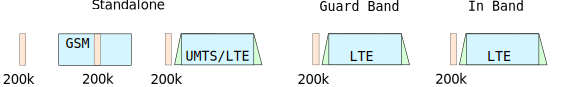
\includegraphics[width=16cm]{nb-iot}
        \caption{Modalità di funzionamento NB-IoT}
\end{figure}
Così facendo operatori di rete i quali possiedono ancora l'infrastruttura gsm,
possono andare a riutilizzarla , diversamente è possibili andare ad adattare le
cellule 4G per renderle compatibili con questa tecnologia.
Quello che si prefigge NB-IoT, e riuscire a garantire la sicurezza delle
comunicazioni cellulari, offrendo un basso costo di sviluppo dal lato hardware,
una lunga durata della batteria, limitando il thruput massimo dei devices.


\subsection{NB-IoT e LTE-M}
Simile ad NB-IoT, LTE-M o LTE Cat-M1  è uno standard che opera su frequenze 
licenziate , della rete 4G. Il vero punto di forza di questa tecnologia è il
poter utilizzare le celle 4G senza dover apportare modifiche, andando ad
offirere una maggiore thruput, a discapito dei consumi energetici. Per questo motivo
LTE-M è in rapida espansione. 

\ref{fig:comparazione_reti}, queste due tecnologie offrono prestazioni diverse,
e si impongono due use-case diversi.
Quindi funzionano in uno spettro proprietario, e forniscono prestazioni diverse
per i diversi use-case. In particolare devices che utilizzano NB-IoT hanno una
durata della batteria molto più prolungata di quelli che utilizzano la
connessione LTE-M, la quale permette un maggiore band-with a discapito delle
durata. Il vantaggio di questi standard e che non servono grandi cambiamenti
alla rete telefonica, quindi sono facilmente implementabili dalle compagnie
telefoniche. Inoltre, ogni devices sarà dotato di una sim-card per poter
connettersi, in questo modo è possibile ottenere  una sicurezza simile a quella
implementato nelle connessioni LTE.
Altro punto a favore è il fatto che non è necessario utilizzare gateway, ogni
devices e connesso direttamente alla rete. 
La maggior parte delle compagnie telefoniche ha già dei piani per rendere disponibile queste due
tecnologie.

\begin{figure}[h]
        \centering 
                \includegraphics[width=11cm]{Comparsion_no_line}
        \caption{Comparazione reti LPWAN}
        \label{fig:comparazione_reti}
\end{figure}

\subsection{Sigfox}
Sigfox, azienda francese la quale dal 2015 ha iniziato a sviluppare una rete
privata in Francia Spagna e Regno unito, promettendo di coprire più di 60 stati
entro il 2020. Sigfox opera sulle frequenze ISM, quindi i costi delle
infrastrutture e i costi che l'utente finale è tenuto a supportare sono molto
inferiori rispetto alle soluzioni che si basano sulla rete cellulare. Il principale,
vantaggio di avere una rete unica mondiale, è la possibilità di un abbonamento unico e la
continuità di funzionamento dei diversi devices in tutte le aree coperte.
Utilizzando una modulazione \emph{Ultra narrow band}, Sigfox, permette di
coprire distanze pari a un paio di chilometri nelle zone urbane, fino a alcune
decine di chilometri in zone rurali. Essendo Sigfox una tecnologia
open hardware, è semplice per i produttori di moduli radio, adattare i loro
componenti per renderli compatibili alla rete Sigfox. In questo modo il costo
per unità diventa molto basso.
Appoggiandosi a frequenze ISM, questa tecnologia è limita la dimensione massima
del payload per messaggio pari a 12 byte, con 140 messaggi inviabili al giorno
per devices.

Per riuscire a gestire in maniera adeguata il sempre maggior numero di device
connessi, e le diverse problematiche che essi comportano, è necessario andare a
ridisegnare la topologia di rete per fare in modo che rispecchi i punti necessari
per garantire il corretto funzionamento. Finora le principali tecnologie
utilizzate erano la rete cellulare 2G, 3G, 4G, la quali hanno un ampia copertura
su tutto il territorio, ma devices che alimentati tramite batteria hanno durate
massime di mesi. Oltre alla rete cellulare abbiamo gli standard IEE 802.11, il
comunemente chiamato wifi, il quale garantisce una copertura di poche decine di
metri e favorisce una connessione veloce a discapito della durata della
batteria. Oppure, Bluetooth e ZigBee i quali hanno offrono una connessione
wireless con copertura di poche decine di metri. Oltre al fatto di una scarsa
copertura e di un elevato consumo di energia per comunicazione, tutte queste
tipologie di rete non sono scalabili cioè non sono ideate per supportare un
carico di milioni di devices connessi contemporaneamente. 

\chapter{Caso di studio}
Con l'evolversi della tecnologia, ed in particolare con l'avvento dell'IoT,
l'aspettativa delle applicazioni basate sul cloud è cambiata. La necessità di
elaborare un numero sempre maggiore di dati ha spinto, sempre più aziende, ad
adottare strumenti cloud based forniti da terzi come ad esempio Microsoft Azure o Amazon
AWS.  Ed è utilizzando questi servizi  che l'architettura classica del
software monolitico ha mostrato i suoi limiti. Con architettura monolitica si
intende una applicazione self-contained indipendente dalle altre
applicazioni presenti nel sistema.  Basandosi su questa modello, ogni
software necessita di essere disinstallato e reinstallato nel momento in cui
sia necessario apportare delle semplici modifiche. Per superare i limiti del
modello monolitico, è stato introdotto il concetto di 
\emph{microservzio}.  La differenza tra una architettura monolitica ed una
basata su microservizi è la  modularità che quest'ultima garantisce.  Prendiamo
come esempio una applicazione formata da un database, un interfaccia web
(client-side user interface)  e una applicazione server (server-side
application).  L'applicazione server-side interpreterà le richieste fatte
dall'utente andando ad eseguire operazioni interne al server, aggiornerà il
database e fornirà il risultato all'utente finale tramite l'interfaccia web.
Nel modello classico  è necessario riscrivere o aggiornare l'intero 
software per apportare delle modifiche o aggiungere delle funzionalità.\\ 
Con il termine \emph{microservices}
si intende una architettura basata su oggetti chiamati \emph{component} ognuno
dei quali fornisce ed utilizza dei \emph{servizi}. Con \textit{component}, si intende
una "parte" di software che può essere aggiornata e sostituita indipendente
dalla applicazione principale.  Ogni \emph{component} si basa sull'utilizzo e la
condivisione di servizi.  I servizi sono l'equivalente delle librerie in una
architettura monolitica, al contrario di queste ultime però, i servizi sono
sviluppabili indipendentemente dalla applicazione principale.
In questo capitolo verrà esposto lo sviluppo di due 
 di applicativi per la gestione e l'interazione di sensori
basti su LoRa, tramite l'utilizzo del framework EveryWare Software Framework ESF
basato su OSGi e sviluppato da Eurotech.
\section{OSGi}
La tecnologia OSGi (Open Services Gateway initiative),
è un insieme di specifiche che definiscono dei componenti
dinamici in grado di estendere le funzionalità dell'ambiente  Java.
Basandosi su di una architettura a microservizi, OSGi permette la gestione in
modo remoto di componenti chiamati Bundle o Deployment Package(dp), i quali
possono essere installati, attivati, aggiornati e fermati senza la necessità di
riavviare l'applicazione principale\\
Ogni bundle è composto dai file contenti le classi ed i metodi specifici per le
funzionalità che implementa e da  metadati utili al framework
per distinguere le classi private da quelle pubbliche. 
Per rendere compatibile questa architettura con il linguaggio di programmazione
Java e la Java Virtual Machine, OSGi ha strutturato il framework su vari
livelli:
\begin{itemize}
        \item   \textit{Bundles}. Bundles sono normali applicazioni JAR contenenti
        \item   \textit{Services}. Il service layer connette in maniera dinamica
                i bundles offrendo un modello publish-find-bind basto su
                l'interfaccia Java POJIs.
        \item   \textit{Services Registry}. Questo layer è composto da una serie
                 API per la gestione dei servizi.
        \item   \textit{Life-Cycle}. Insieme di API per gestire \hyperlink{cycle_bundle}{il ciclo vitale
                dei bundle}
        \item   \textit{Modules}. È il layer che definisce in che modo i bundle
                sono in grado di interagire importando ed esportando pezzi di
                codice.
        \item   \textit{Security} È un layer che opera su tutti i livelli e
                garantisce la sicurezza delle applicazioni OSGi andando a
                limitare le funzionalità del bundle.
\end{itemize}
\begin{figure}[th]
\centering 
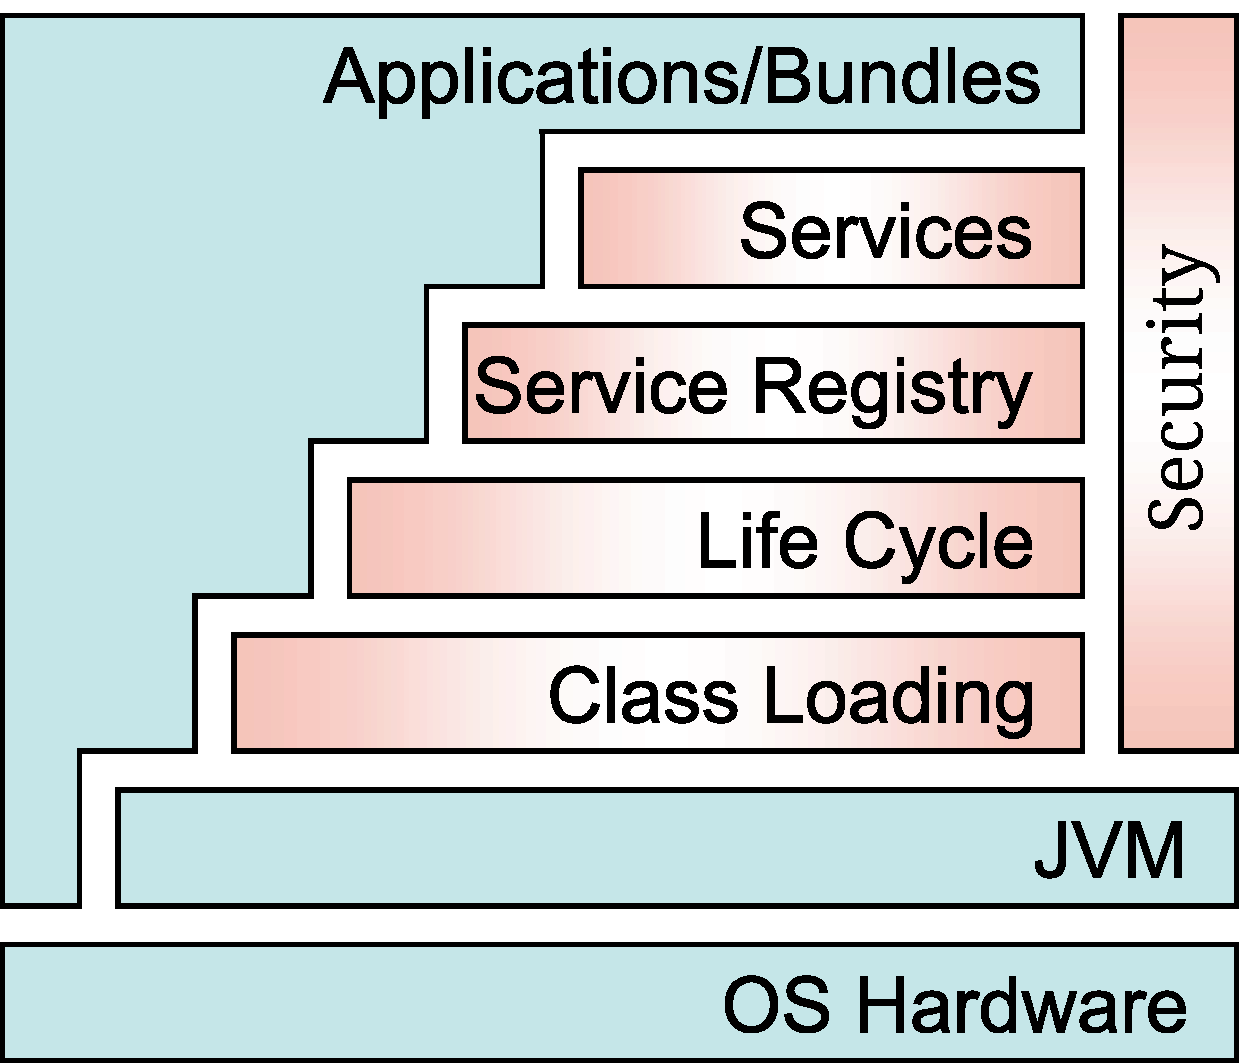
\includegraphics[width=10cm]{osgi}
\caption{Layer OSGi}
\label{}
\end{figure}

\subsection{Ciclo vitale dei bundle}\hypertarget{cycle_bundle}{}
In un modello così dinamico, è necessario che il framework sia basato su di un
software fail-safe in grado di gestire le eccezioni che si possono verificare
durante l'installazione e disinstallazione di nuovi moduli.
Non è raro infatti che nuovi bundle ,installati nel sistema, richiedano servizi
non ancora disponibili o attualmente utilizzati da altri componenti.
Per far fronte ai problemi riscontrabili, OSGi assegna ad ogni  i bundle  uno 
\emph{stato} tra:
\begin{itemize}
        \item   \textit{Installed} Il bundle è stato installato nel sistema, ma
                non sono presenti alcune delle sue dipendenze.
        \item   \textit{Resolved} Il bundle è installato e le sue dipendenze
                presenti nel sistema.
        \item   \textit{Starting} Uno stadio temporaneo attraverso il quale il
                bundle passa prima di essere attivato.
        \item   \textit{Active} Il bundle è stato correttamente attivato e sta
                eseguendo le sue funzioni all'interno del sistema.
        \item   \textit{Stopping} Uno stadio temporaneo in cui il bundle passa
                prima di essere disattivato.
        \item   \textit{Uninstalled} Il bundle è stato rimosso dal container
                OSGi
\end{itemize}

\subsection{Module layer}
Il module layer è dove il framework OSGi gestisce la "modularità" di un bundle.
È in questo layer che vengono processati i metadati contenuti all'interno del
file MANIFEST.MF. Tramite questo file il framework OSGi è in grado di
determinare le dipendenze del bundle e quali servizi è in grado di esportare.

\subsection{Registrazione del servizio}
Un \emph{servizio} in OSGi è definito tramite una classe Java standard. Per
implementare un nuovo servizio, è necessario definire quale classe o quale
interfaccia si vuole fornire il servizio.
La soluzione a questo, è l'utilizzo di registri di servizio. Ogni bundle può
esporre dei metodi ed registrarli attraverso il service registry. In questo
modo, altri bundle possono accedere al service registry e utilizzare i metodi
listati nel registro. Un bundle quindi può registrare un servizio, può
utilizzare un servizio oppure può mettersi in attesa aspettando che un servizio
venga registrato o eliminato.
Inoltre i servizi sono dinamici, ogni bundle può mettersi in lista per
richiedere un servizio mentre altri stanno ancora utilizzando il servizio.
\begin{figure}[th]
        \centering 
                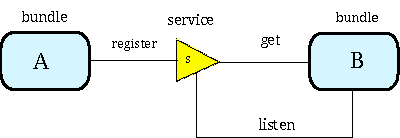
\includegraphics[width=9cm]{osgi_service}
        \caption{Schema utilizzo servizi OSGi}
        \label{}
\end{figure}

\section{Everyware Software}
ESF o Everyware Software è un framework che si interpone tra il sistema operativo
e le applicazioni utente. Basato su Java/OSGi, ESF si pone l'obiettivo di
offrire  la possibilità di sviluppare applicativi, per il mercato M2M ,in maniera semplice e veloce
. Ideato per operare all'interno di gateway
industriali, fornisce al consumatore servizi e librerie per l'accesso delle più
comuni porte di comunicazione RS232/485, GPIO, CAN.
ESF tramite la sua interfaccia web, permette di controllare da remoto il
comportamento dei gatway.
\ref{fig:ESF_web}.
%\begin{figure}[th]
%        \centering 
%                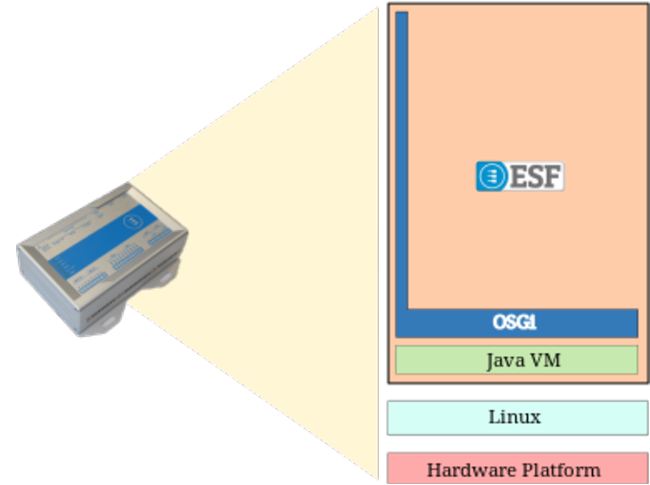
\includegraphics[width=10cm]{ESF_layer.pdf}
%        \caption{OSGi services}
%        \label{}
%\end{figure}


\begin{figure}[th]
        \centering 
                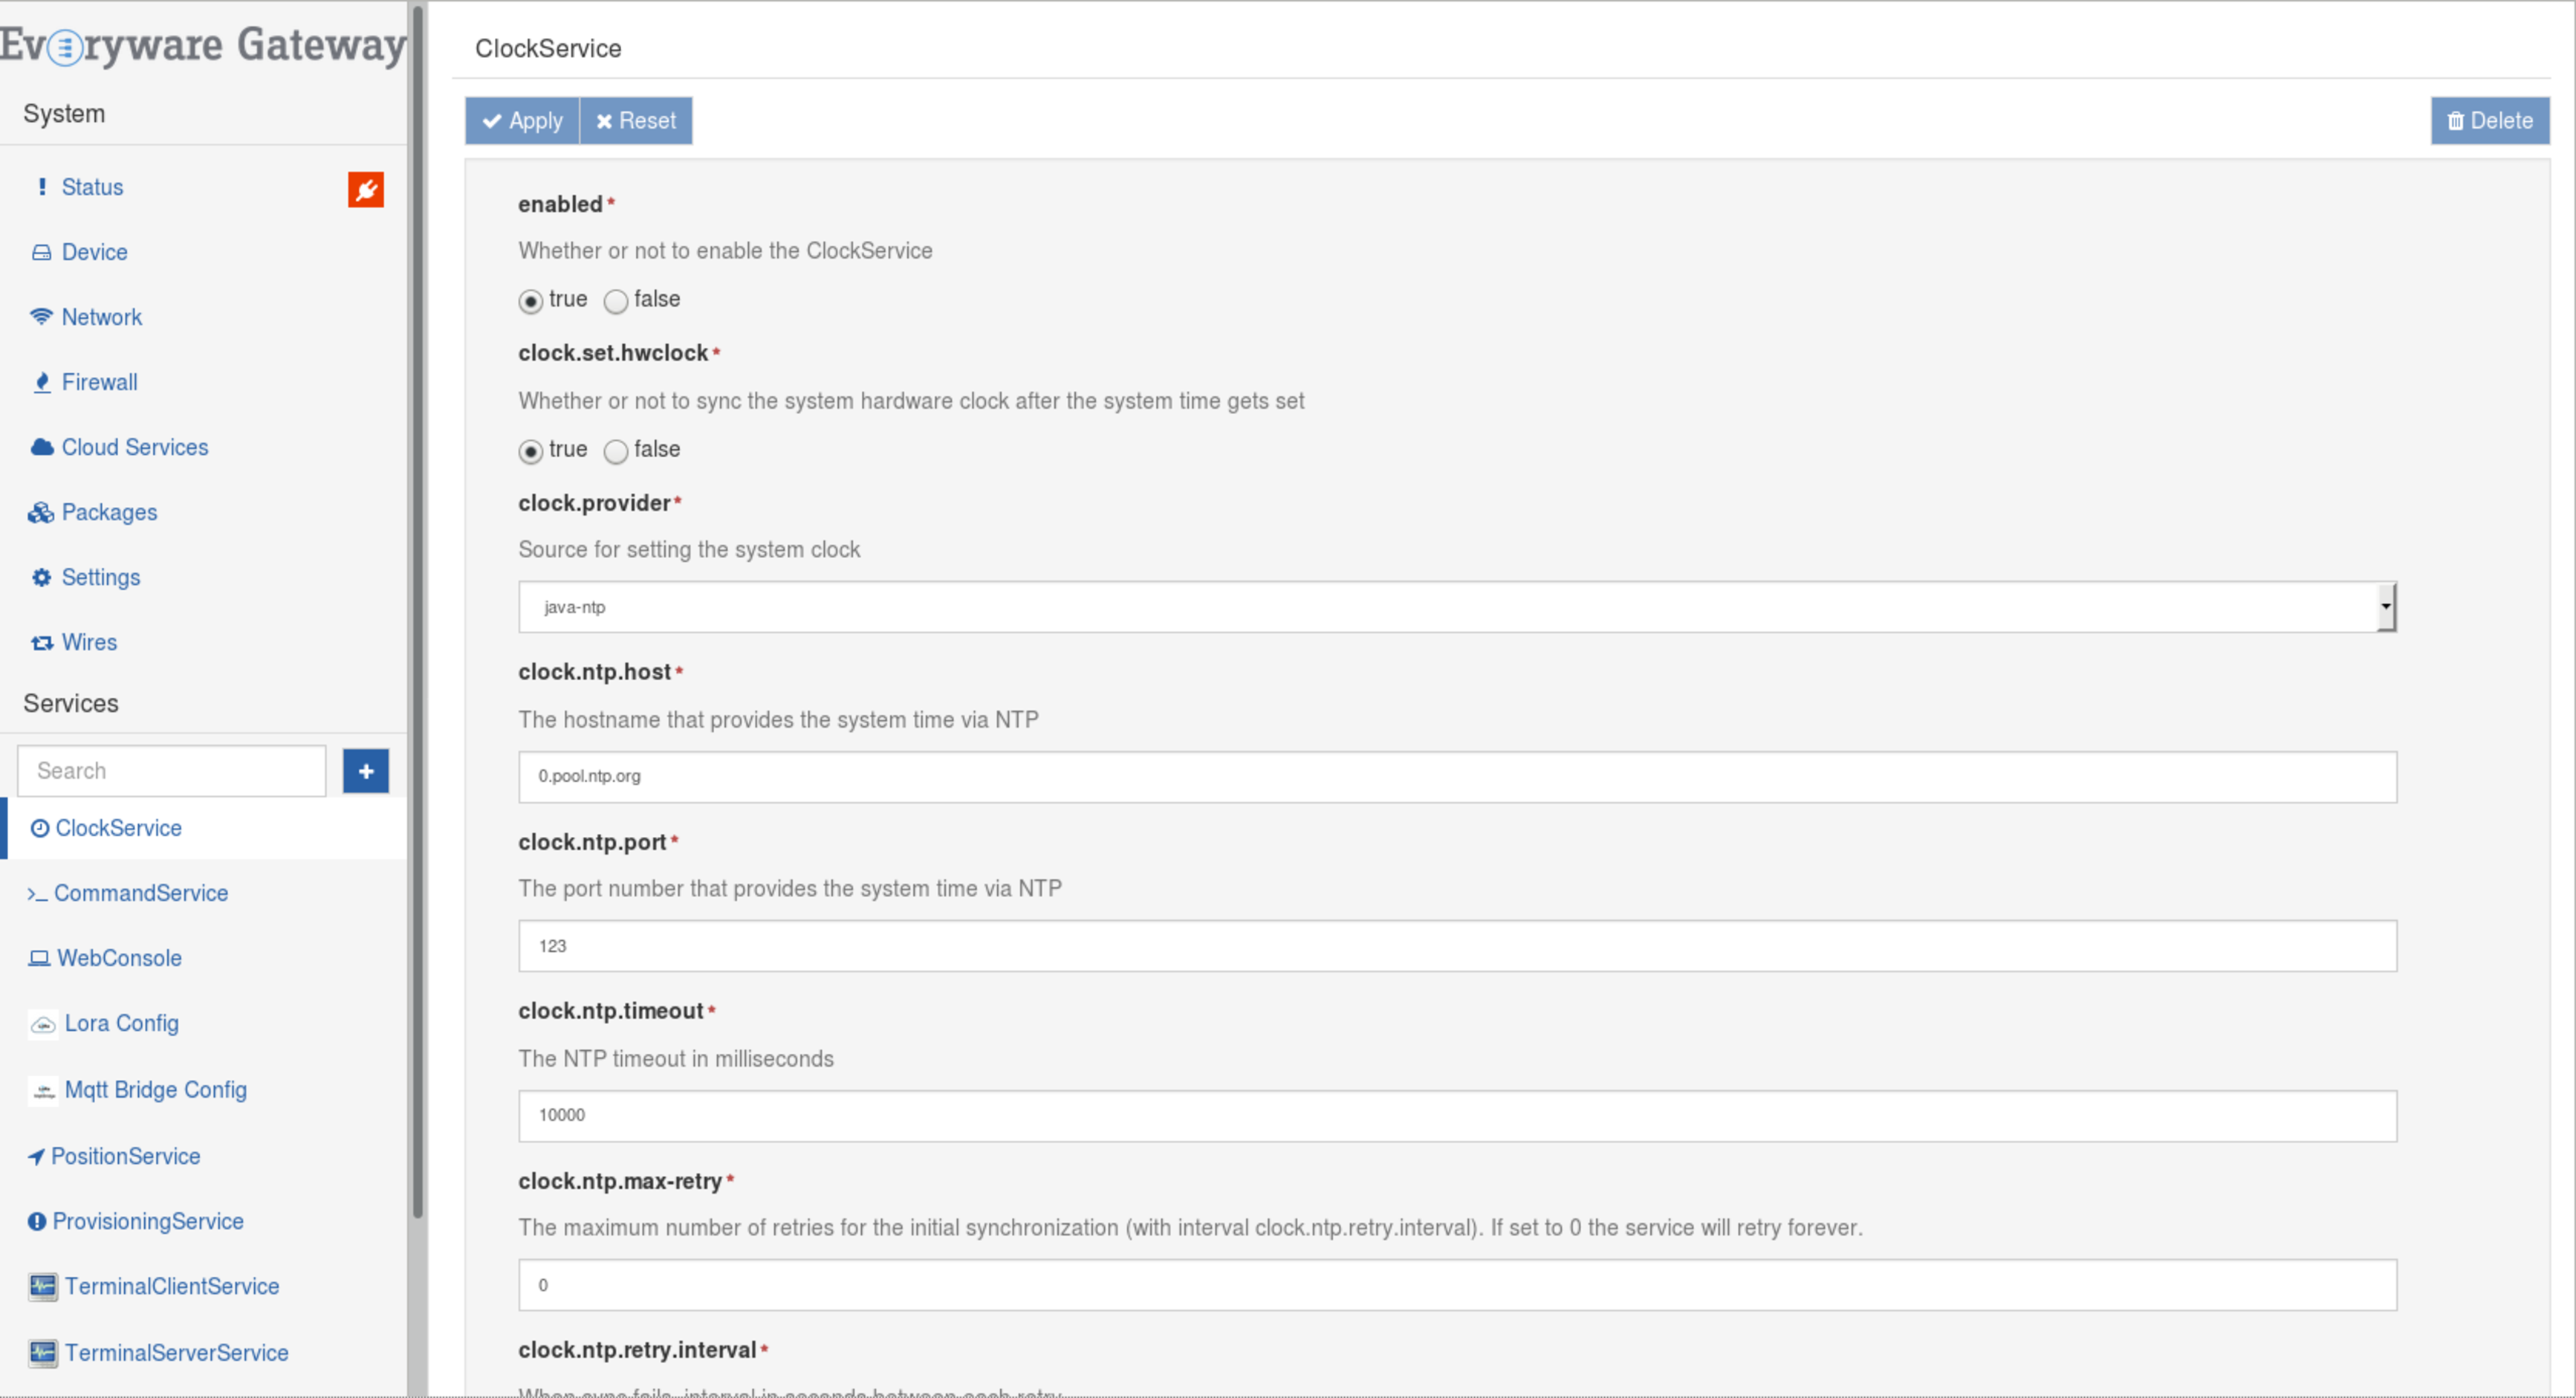
\includegraphics[width=12cm]{ESF.png}
                \caption{Interfaccia web ESF}
        \label{fig:ESF_web}
\end{figure}

\pagebreak


\section{Architettura del software}
Per integrare ESF con il ricevitore lora SX1301, è stato necessario l'utilizzo
di due software aggiuntivi.
Il primo è LoRa packet forwarder fornito da Semtech. Questo
applicativo permette di comunicare con le periferiche di basso livello presenti
nel ReliaGATE 10-11 in modo da astrarre ad un più alto livello i dati ricevuti dal
ricevitore .
L'altra applicazione utilizzata, è LoRa Gateway Bridge. Tramite questa
applicazione è stato possibile 
reindirizzare i dei dati forniti dal packet forwarder ad un server MQTT.

\begin{figure}[th]
        \centering 
                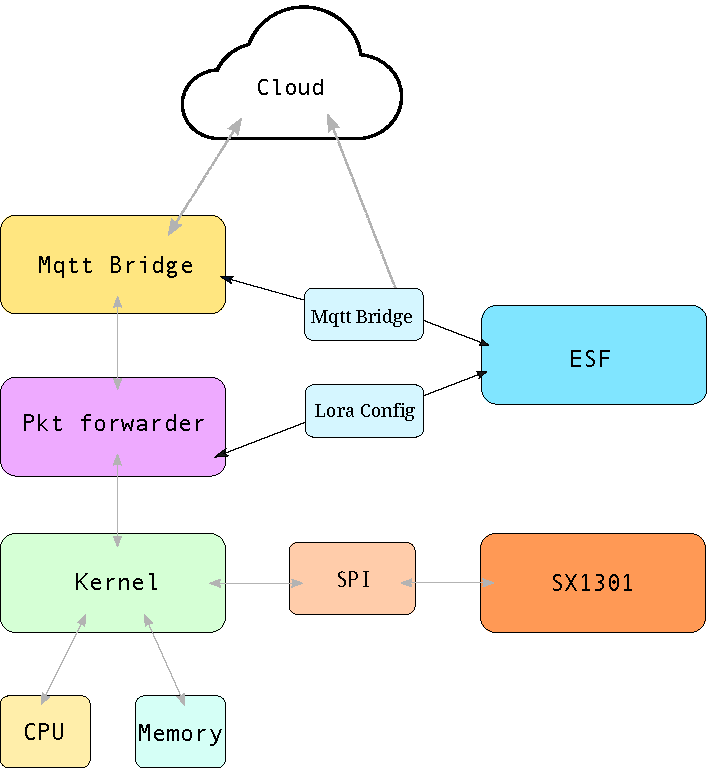
\includegraphics[width=11cm]{Application_layer}
        \caption{Architettura del software}
        \label{fig:Software_stack}
\end{figure}

\subsection{Semtech packet forwarder}
Il packet forwarder è un software che permette la ricezione e l'invio di pacchetti radio Lora ,
tramite una connessione SPI con il device SX1301. Nel caso di ricezione di un
pacchetto, l'applicativo incapsula i dati ricevuti in un formato UDP, e li
ritrasmette nella rete internet/intranet. Per la sua configurazione viene
utilizzato un file Json nel quale troviamo tutte le varie opzioni di
configurazione per i moduli radio presenti al interno del chip.
\inputminted[mathescape, gobble=2, frame=lines, linenos=true
framesep=2mm, firstline=1,lastline=23]{json}{Code_Files/global_json.conf}
\inputminted[mathescape, gobble=2, frame=lines, linenos=true
framesep=2mm, firstline=173,lastline=184]{json}{Code_Files/global_json.conf}

\subsection{LoRa Gateway Bridge}
LoRa Gateway Bridge è un applicativo in grado di identificare i vari pachetti UDP inviati
dal packet forwarder e inotrarli ad un Broker MQTT. 
Il software è scritto nel linguaggio GO e permette una configurazione tramite
linea di comando.  Per renderlo interfaciabile con ESF, sono state apportate delle 
modifiche al codice; in particolare è stata aggiunta la possibilità di
specificare il publish e il subscribed topic, i quali erano hard-coded.
%\inputminted[mathescape, gobble=2, frame=lines, linenos=true
%framesep=2mm, firstline=1,lastline=23]{go}{Code_Files/bridge_mqtt.go}
Il codice sottostante, rappresenta un esempio di pacchetto LoRa inoltrato dal
LoRa Gateway Bridge ad un broker MQTT
\inputminted[mathescape, gobble=2, frame=lines, linenos=true
framesep=2mm, firstline=1,lastline=23]{json}{Code_Files/message.json}
\section{Hardware utilizzato}

\subsection{SX1301}
Per la ricezione dei pacchetti LoRa, è stato utilizzato il chip SX1301 prodotto
da Semtech e collegato al gateway ReliaGate 10-11.
\subsubsection{Struttura interna}
Per quanto riguarda la struttura interna del modulo radio, non si hanno molte
informazioni dato che la tecnologia è proprietaria di Semtech. Nella
documentazione ufficiale è presente una rappresentazione grafica dei vari
blocchi interni al chip.

\begin{figure}[th]
        \centering 
                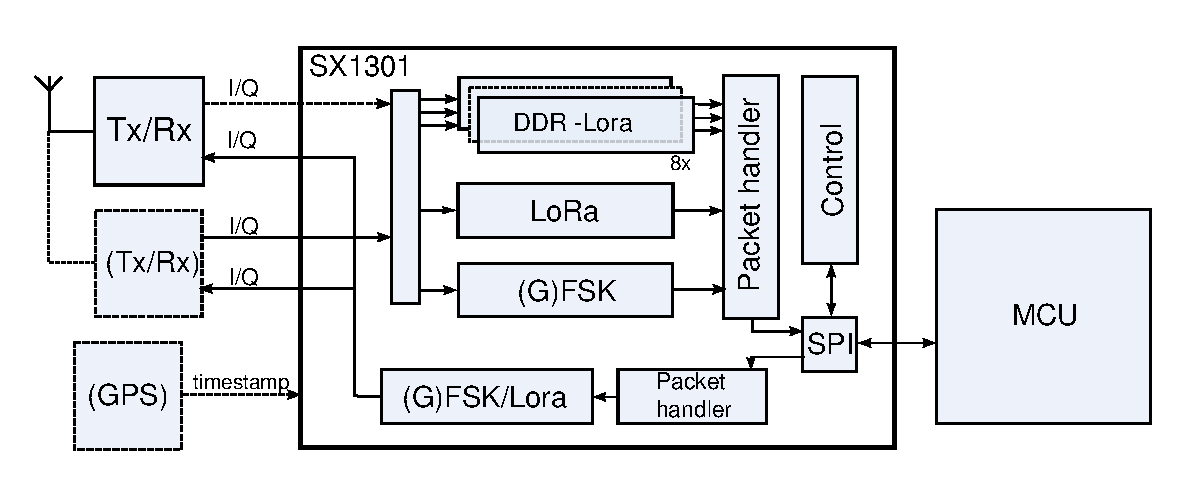
\includegraphics[width=11cm]{SX1301}
        \caption{Struttura interna ricevitore SX1301}
        \label{fig:sx1301}
\end{figure}

Come scritto nella documentazione  \improvement{inserire link} e intuibile dalla
figura \ref{fig:sx1301} il chip è in grado di scansionare contemporaneamente 
8 canali diversi (IF0 a IF7)  permettendoli di rimanere in ascolto per garantire
la ricezione dei segnali con SF diversi.
Inoltre data la quasi ortogonalità degli Spreading Factor
, il chip è in grado di ricevere un pacchetto
con uno Spreading Factor $i$ anche nel caso in cui si sovrapponga ad un altro
pacchetto con Spreading Factor pari a $j$, fintanto che $i\neq j$. Questa
pseudo-ortogonalità utilizzata in LoRa, permette al ricevitore  SX1301 
di demodulare fino ad un massimo di 8 pacchetti contemporaneamente.
Nella tabella \ref{tab:sx1301_spec} sono riportate le caratteristiche elettriche
massime del  chip SX1301. Il Chip, supporta tensioni di
alimentazione fino a 4V e  come e possibile osservare il range di temperatura in cui il
chip può operare è molto ampio, rendendolo ideale per applicazioni esterne ed
interne. 

\begin{table}[th]
        \centering 
                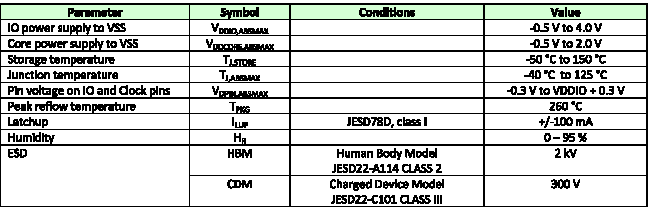
\includegraphics[width=16cm]{SX1301_table}
        \caption{Caratteristiche elettriche SX1301}
\label{tab:sx1301_spec}
\end{table}
Utilizzando i valori nominali riportati nella tabella \ref{tab:sx1301_spec_1},
si hanno valori di corrente pari a 1[uA] in idle  e di 5[mA] in pieno
funzionamento.
\begin{table}[th]
        \centering 
                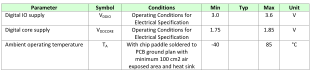
\includegraphics[width=16cm]{SX1301_table_1}
        \caption{Caratteristiche elettriche SX1301}
        \label{tab:sx1301_spec_1}
\end{table}
Per la ricezione del segnale è stata utlizzata una antenna omnidirezionale,
ideata per la banda degli 868[MHz] con un guadagno pari a 3[dB].
\subsection{ReliaGATE}
Il gateway a cui è collegato il modulo SX1301 è il ReliaGATE 10-11 prodotto da
Eurotech. Al suo interno troviamo un processore Texas Instruments TI AM335X Cortex-A8 
equipaggiato con 512MB di RAM e 4GB di storage eMMC. Il ReliaGATE offre una
vasta gamma di porte tra cui 232/485, 2CAN bus, 2 porte USB e 2 porte Ethernet,
inoltre ha connettività Bluetooth, WiFi e GPS. Al suo interno è installo
Everyware™ Software Framework (ESF) versione 5.
\begin{figure}[th]
        \centering 
                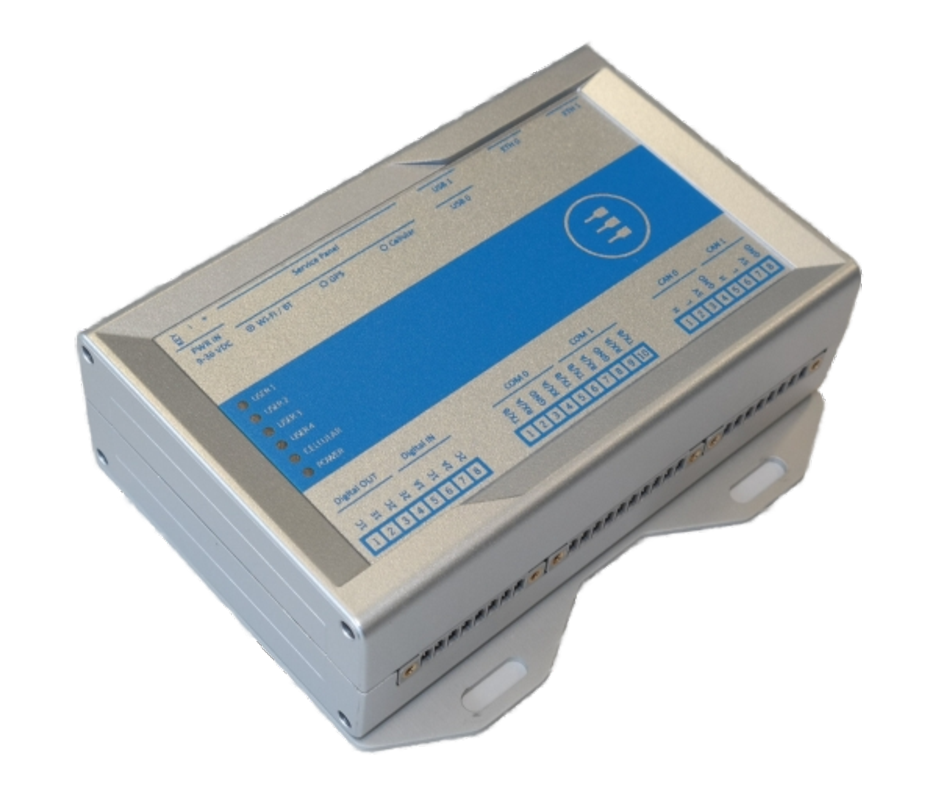
\includegraphics[width=11cm]{Reliagate_10_11}
        \caption{ReliaGATE 10-11}
        \label{fig:ReliaGATE}
\end{figure}



\section{Realizzazione}

Per gestire i due software preinstallati si è optato per la creazione di due
applicativi osgi distinti Lora Config e Mqtt Bridge.
\subsection{Lora Config}
Il primo applicativo chiamato Lora Config si pone il compito di leggere ed
interpretare il file di configurazione utilizzato dal programma \emph{Packet
Forwarder}, per poi andare ad esporre i parametri principali all'utente tramite
l'interfaccia web di ESF.
La libreria utilizzata per manipolare i file di tipo Json è 

\mint{Java}|import com.eclipsesource.json|

Tramite la quale vengono riempiti i campi della classe LoraSettings. Il file
Json è composto da due parti. Nella prima parte
troviamo tutte le impostazioni per la configurazione dei canali (IF0 a IF7)
, nella seconda
parte sono presenti le impostazioni per il forward dei pacchetti. 
Per semplificare la gestione del bundle, sono state create due classi distinte
SX1301Configuration e GatewayConfiguration, accessibili tramite la classe LoraSettings.

\begin{minted}[linenos=true, numbersep=5pt, gobble=2, frame=lines, %
framesep=2mm]{java}
    public class LoraSettings {
            public static final String KEY_GATEWAY_CONFIG = "gateway_conf";
            public static final String KEY_SX1301 = "SX1301_conf";
            private SX1301Configuration sx1301Conf;
            private GatewayConfiguration gatewayConf;
       } 
\end{minted}

Per applicare le modifiche apportate alla configurazione, è necessario che
il packet forwarder venga riavviato. Per eseguire questa operazione si è scelto di
utilizzare la libreria 
\mint{Java}|import com.apache.commons.exec|
la quale fornisce delle API per chiamare processi esterni, in particolare
si è scelto di utilizzare l'utility di sistema \emph{pkill} per terminare il
processo del pkt forwarder.
\begin{minted}[linenos=true, numbersep=5pt, gobble=2, frame=lines, %
framesep=2mm]{java}
          public void startPktForwarder() {
                DefaultExecutor pktExecutor = new DefaultExecutor();
                CommandLine pktCmdLine = new CommandLine(KEY_PKT_BIN);
                pktCmdLine.addArgument("start");
                pktExecutor.setExitValue(0);
                try {

                    pktExecutor.execute(pktCmdLine);
                    s_logger.info("start PKT");
                } catch (Exception e) {
                    s_logger.warn("Coulden't start pkt forwarder");
                }
            }

            public void stopPktForwarder() {
                DefaultExecutor pktExecutor = new DefaultExecutor();
                CommandLine pktCmdLine = new CommandLine("pkill");
                pktCmdLine.addArgument("basic_pkt_fwd");
                pktExecutor.setExitValue(0);
                try {

                    pktExecutor.execute(pktCmdLine);
                    s_logger.info("Stop PKT");
                } catch (Exception e) {
                    s_logger.warn("Coulden't stop pkt forwarder");
                }
        }

\end{minted}

%\begin{figure}[th]
%        \centering 
%        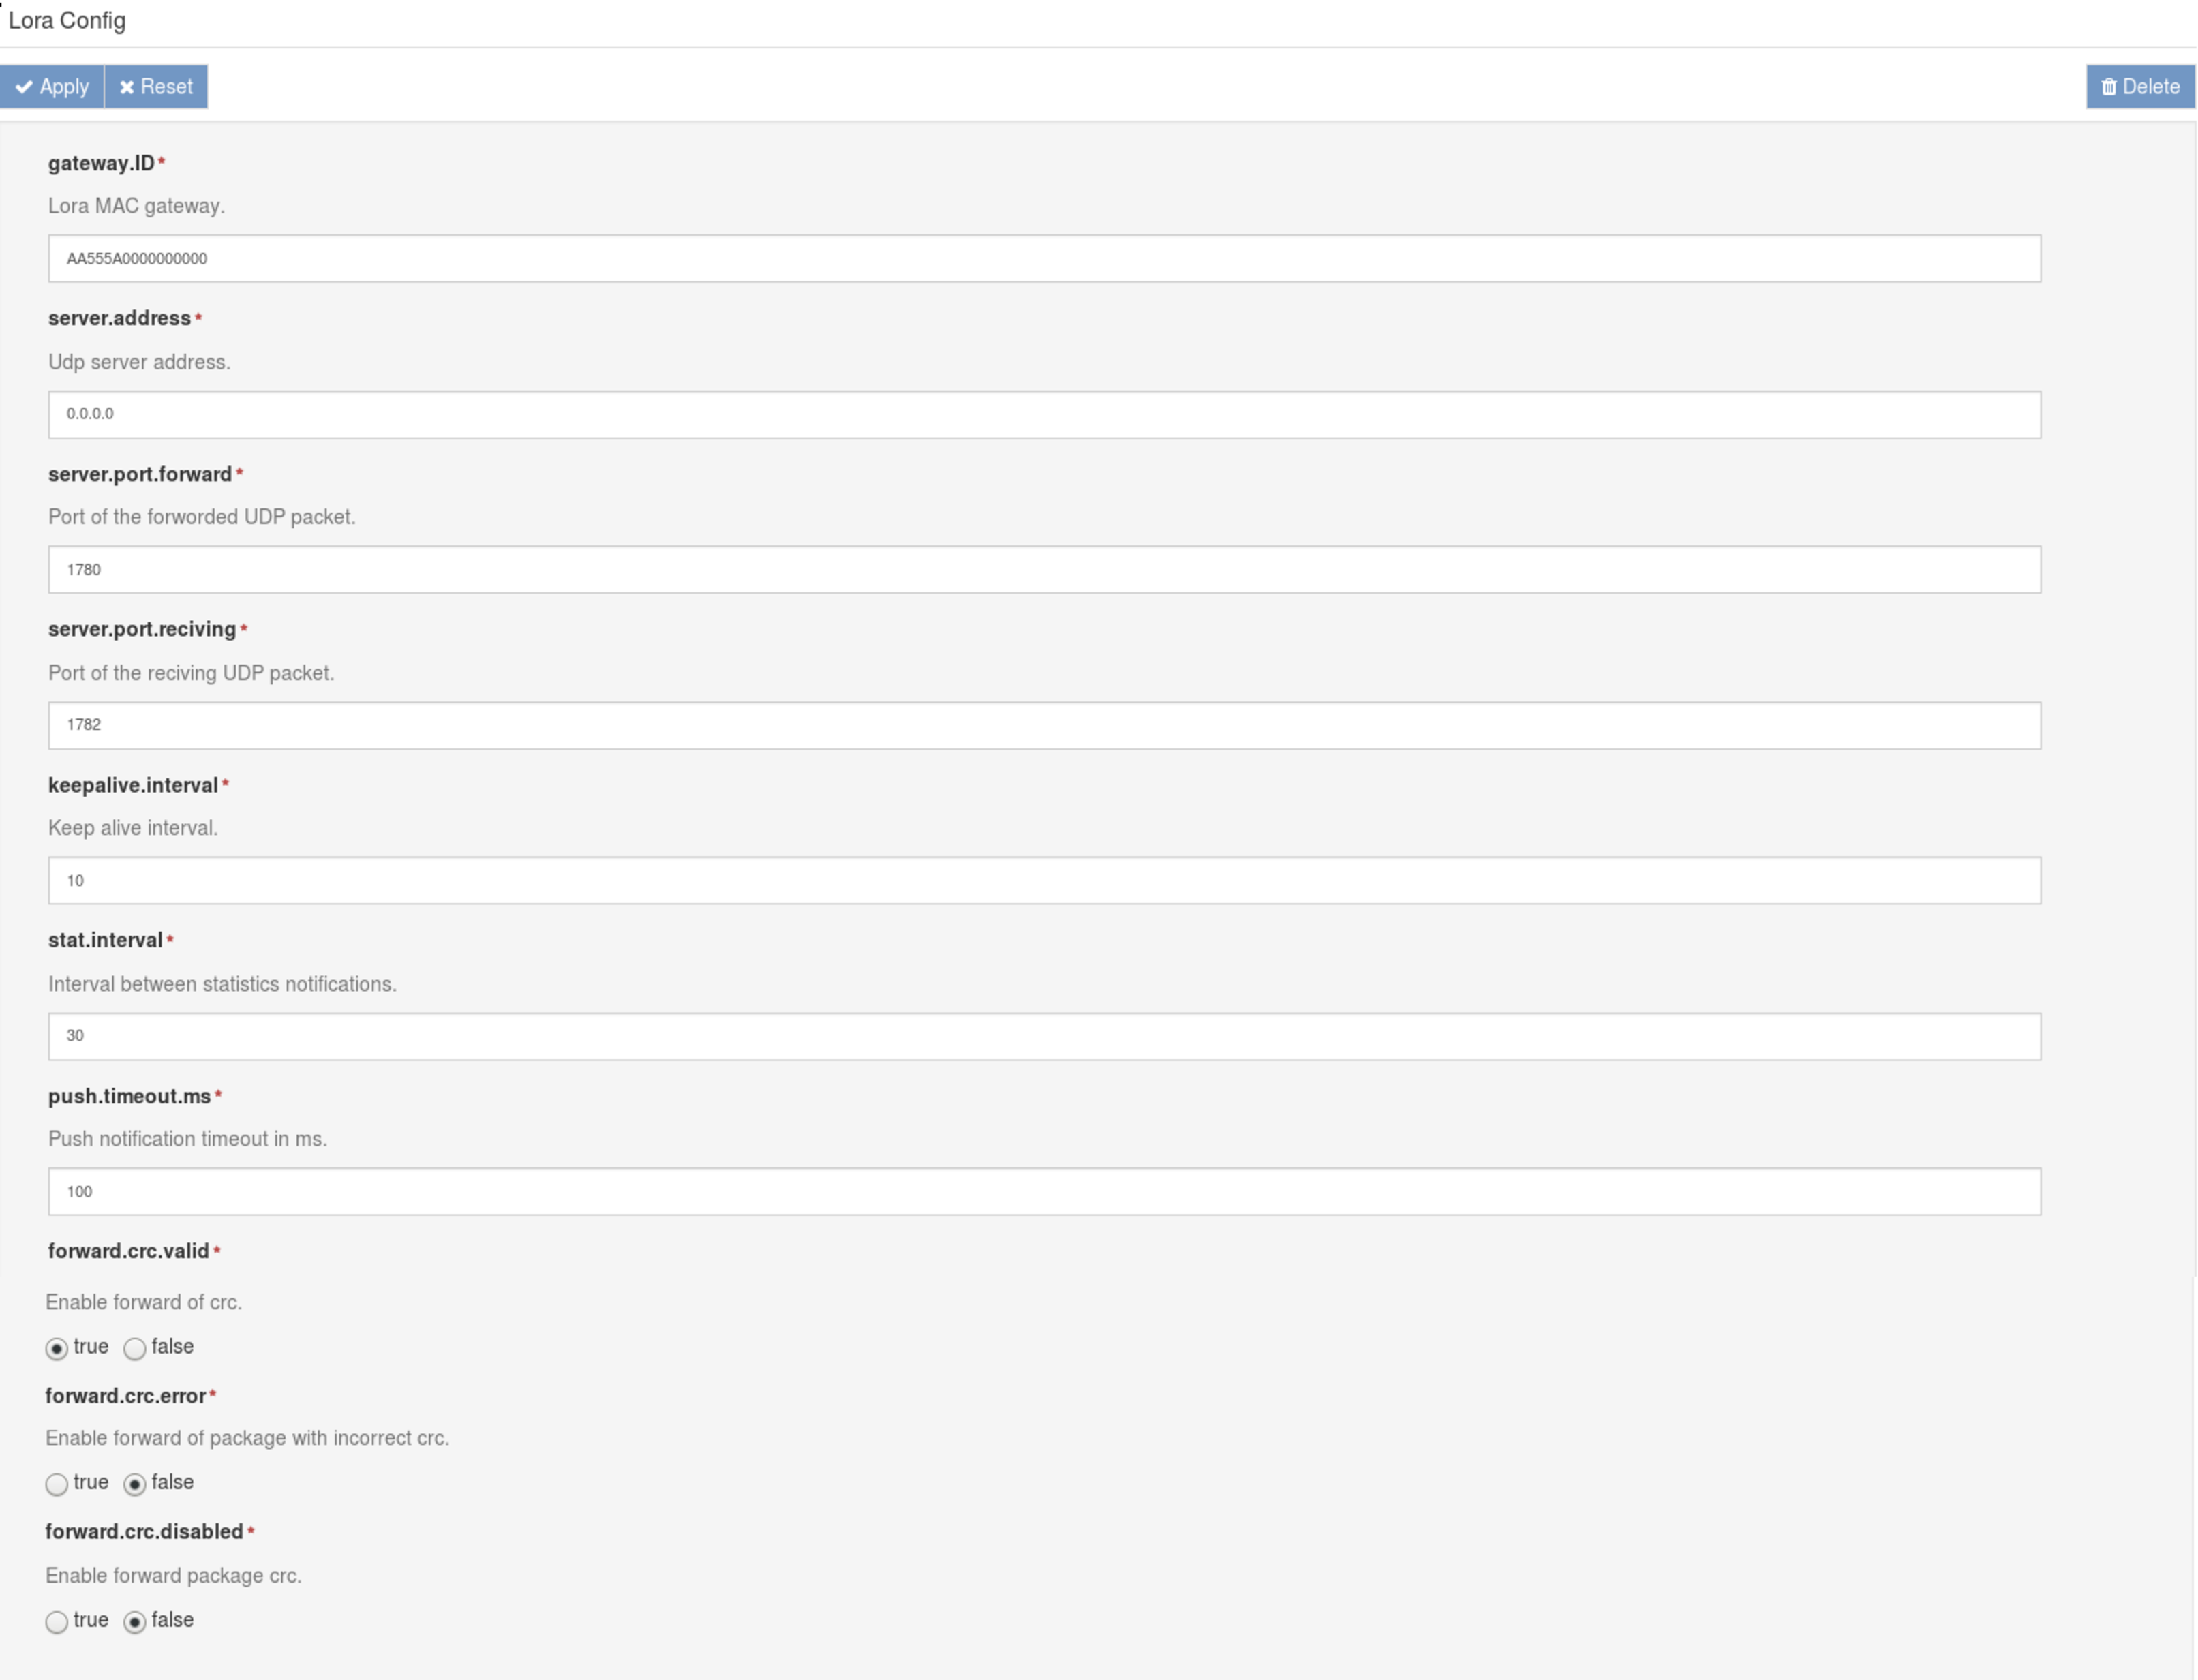
\includegraphics[width=16cm]{Lora_Config}
%                \caption{Architettura del software}
%        \label{fig:Software_stack}
%\end{figure}



\subsection{Mqtt Bridge Config}
Il secondo bundle prende il nome di MQTT Bridge Config e ha lo scopo 
di esporre , tramite l'interfaccia web di ESF, le varie opzioni a linea di
comando dell'applicativo
 \emph{Lora Gateway Bridge}.  Anche in questo caso è necessario il
riavvio del applicativo per fare in modo che le modifiche abbiano effetto. 
Come nel bundle precedente è stata usata la libreria

\mint{Java}|import com.apache.commons.exec|

Tramite l'interfaccia web è possibile modificare i seguenti parametri:
\begin{itemize}
\item il topic sul quale pubblicare i messaggi ricevuti in formato UDP dal
\emph{pkt forwarder}.
\item il topic al quale rimanere il gateway dovrà rimanere in ascolto .
\item su quale indirizzo e porta mandare/ricevere i pacchetti UDP.
\item a quale broker MQTT iscriversi.
\item l'username e password per connettersi al broker.
\end{itemize}

%\begin{figure}[th]
%        \centering 
%                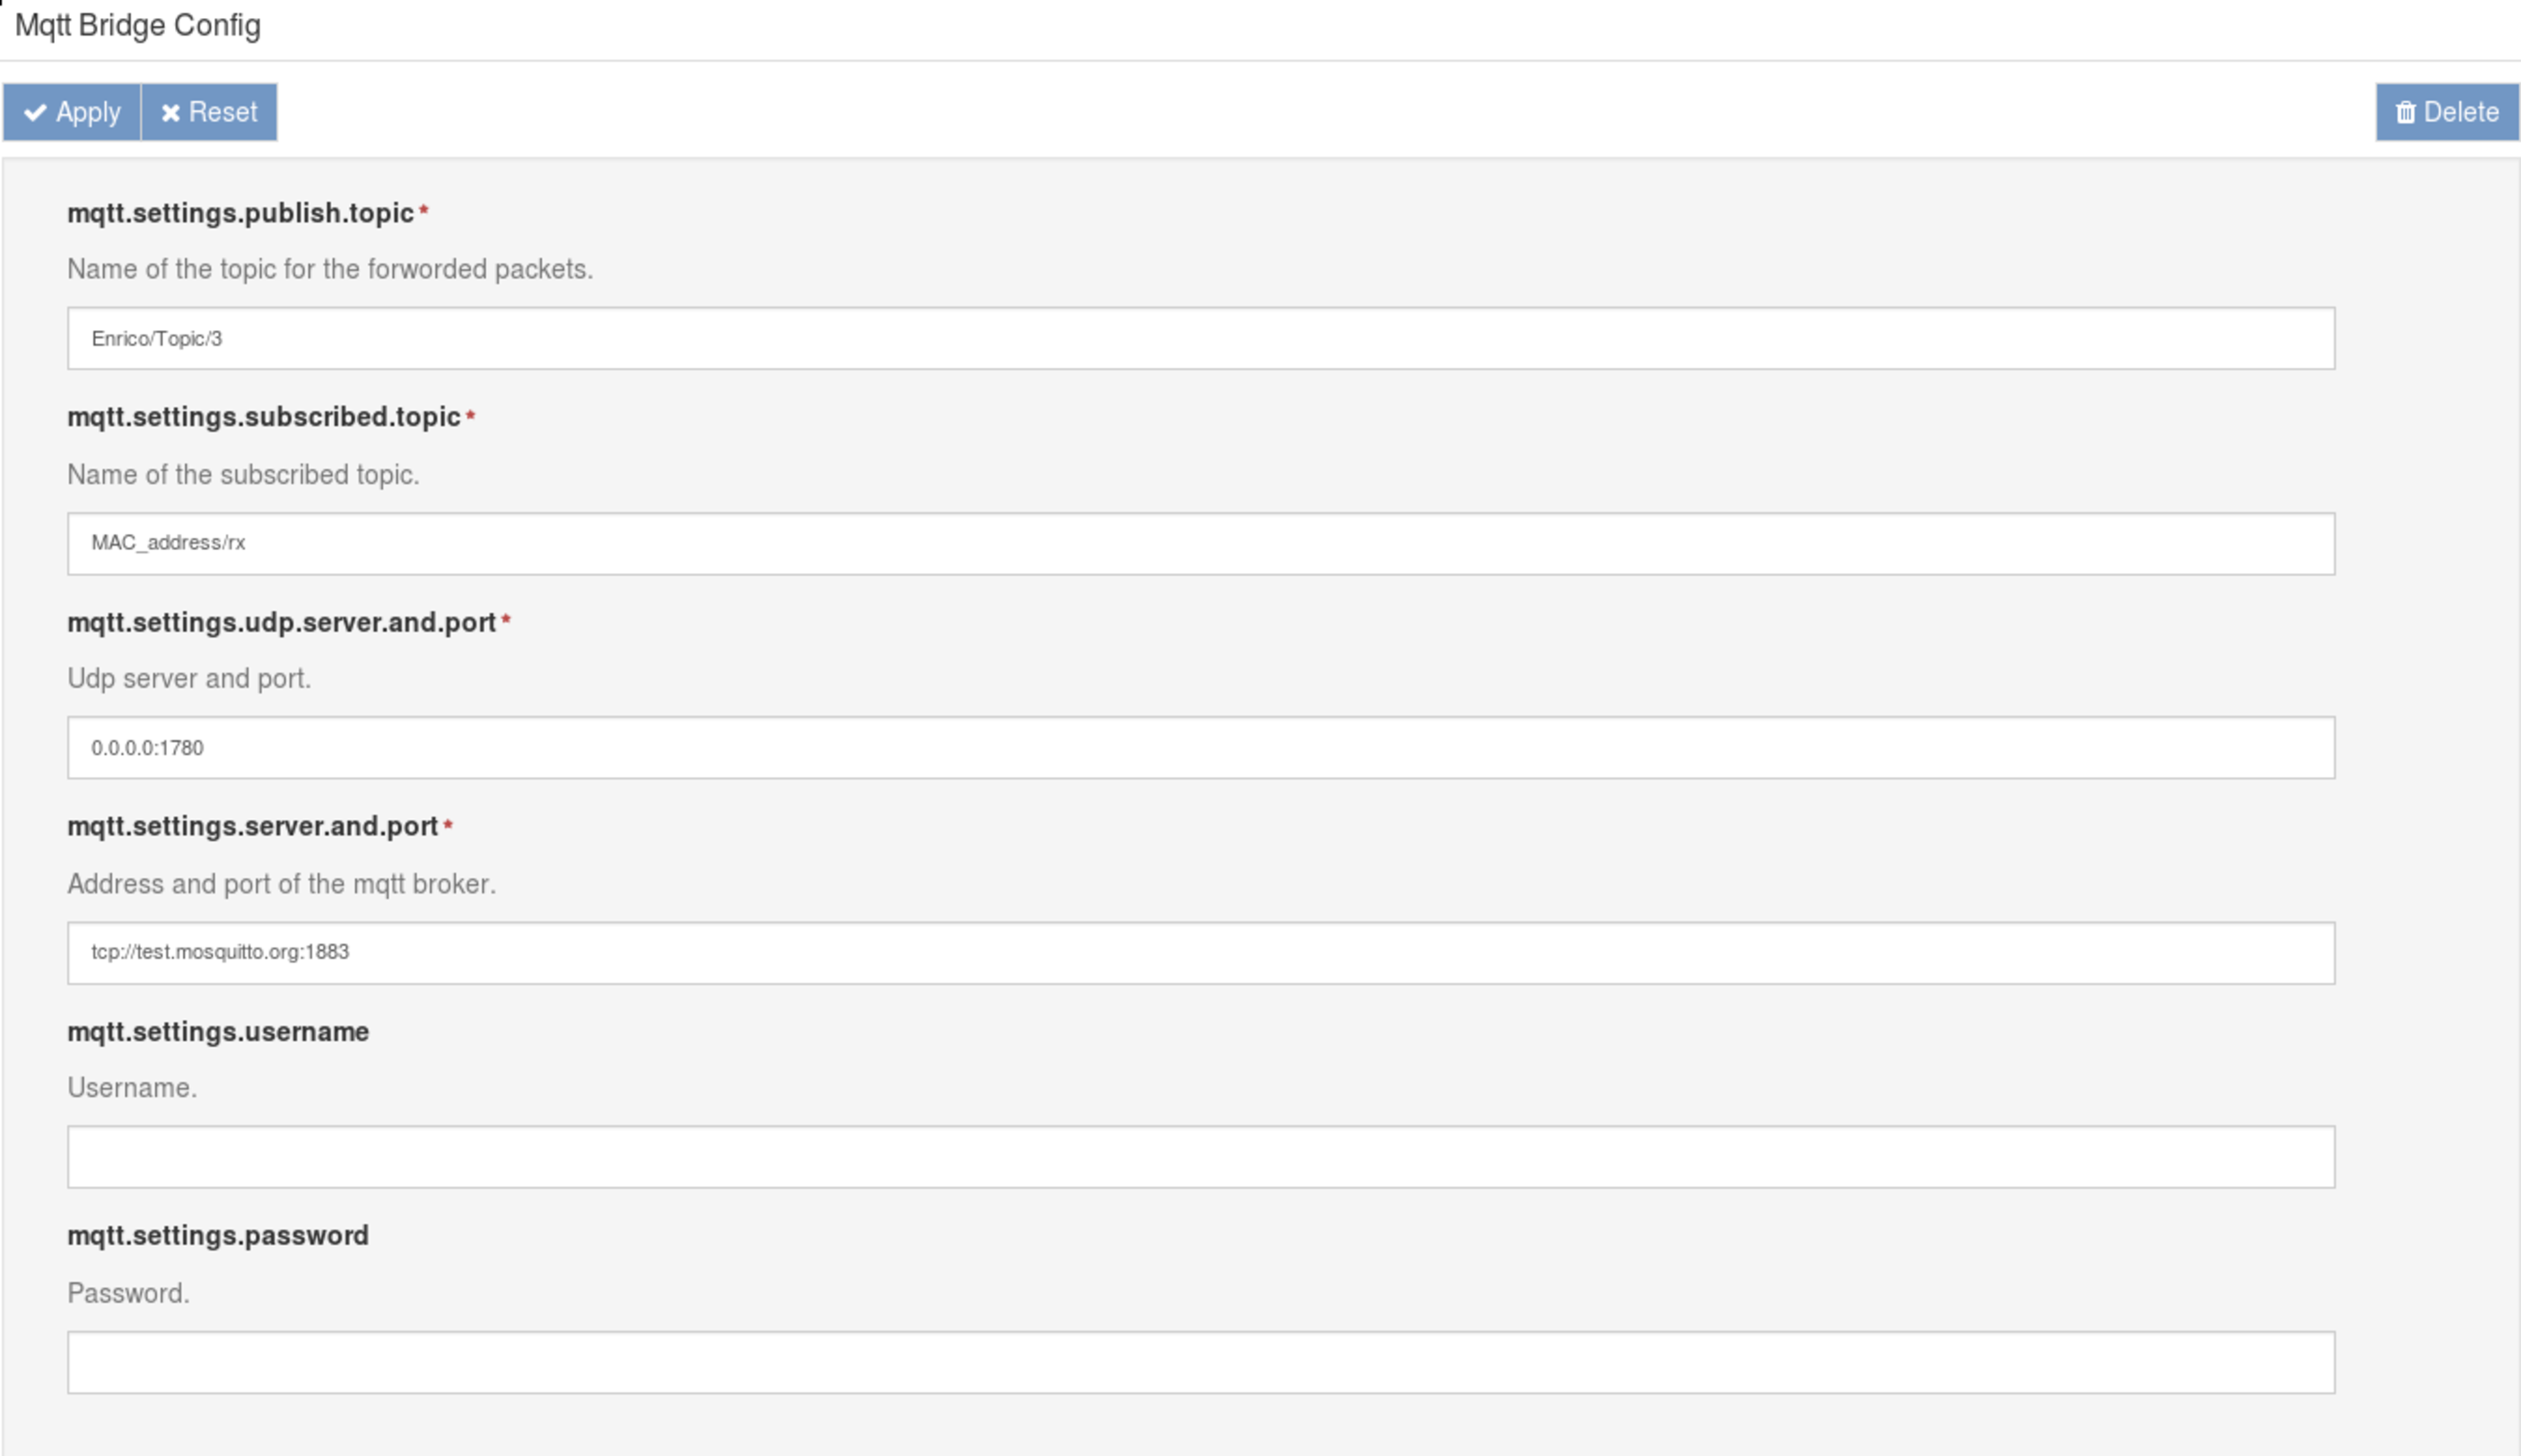
\includegraphics[width=16cm]{Mqtt_Bridge_Config}
%        \caption{Architettura del software}
%        \label{fig:Software_stack}
%\end{figure}

\section{Misurazioni}
Finito lo sviluppo dei bundle, si è scelto di testare la distanza massima
di comunicazione raggiungibile dall'hardware in possesso. 
Il device utilizzato per l'invio dei pacchetti LoRa è prodotto dalla Semtech e
prende il nome di LoRa Mote.
\begin{figure}[th]
        \centering 
                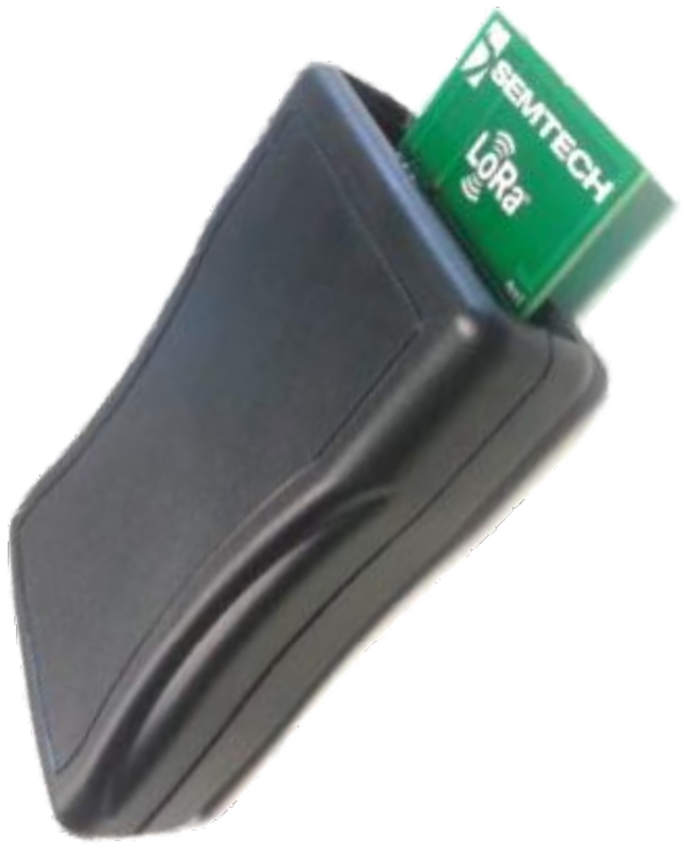
\includegraphics[width=4cm]{LoRaMote_no_wave}
        \caption{Dispositivo LoRa Mote}
        \label{fig:Software_stack}
\end{figure}
In via sperimentale è stato installato  il gateway
ReliaGATE 10-11 ad una altezza di circa 11m. La prova di ricezione è stata condotta per
tentativi cercando , per quanto possibile, di testare diversi punti distribuiti
alla stessa distanza radiale. 
\begin{figure}[th]
        \centering 
                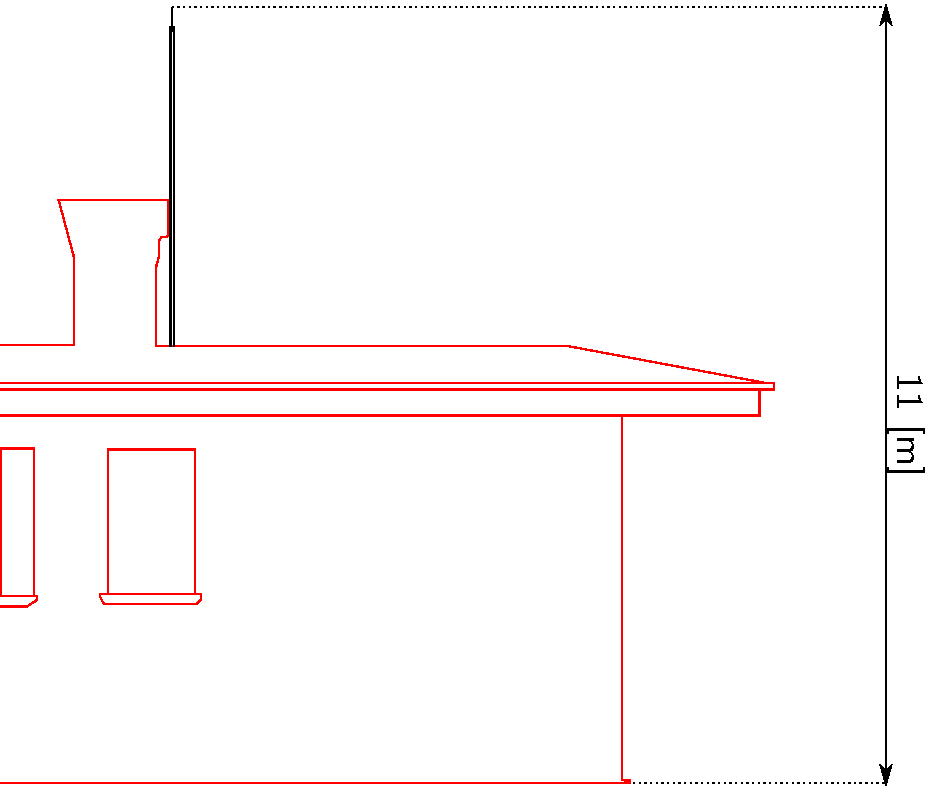
\includegraphics[width=10cm]{casa}
        \caption{Installazione dell'antenna}
        \label{fig:Software_stack}
\end{figure}
Per constatare l'avvenuta ricezione del
messaggio è stata utilizzata l'applicazione Android gratuita \href{
https://play.google.com/store/apps/details?id=at.tripwire.mqtt.client&hl=en}{My
MQTT}, tramite la
quale è possibile iscriversi ad un topic predefinito ed rimanere in ascolto dei
messaggi pubblicati in esso. 
Come broker MQTT si è scelto di utilizzare il
broker open source \href{http://mosquitto.org/}{"mosquitto.org"}. 
\subsection{Osservazioni}

\begin{figure}[th]
        \centering 
                \includegraphics[width=16cm]{map}
        \caption{Copertura Lora}
        \label{fig:map}
\end{figure}
Nella mappa ogni colore corrisponde ad un livello  RSSI ( Received
Signal Strength Indicator) con cui il quale il messaggio inviato in quel punto 
è stato ricevuto.
Dovendo testare la massima distanza di comunicazione, l'algoritmo ADR è stato disattivato,
permettendo così al device di non cambiare configurazione durante i vari test.
LoRa Mote è stato configurato 
per l'invio di messaggi con uno Spread Factor pari a 12 e una larghezza
di banda pari a 125[Khz]. L'ambiente circostante
al luogo dove l'antenna è stata situata è un ambiente suburbano pianeggiante.
La distanza massima raggiunta varia di alcuni chilometri in base alla
conformazione del territorio. In assenza di edifici in linea d'aria tra gateway
e il dispositivo LoRa Mote, è stato possibile ricevere correttamente un 
pacchetto alla distanza di 8,2[Km].
Per quanto concerne i risultati ottenuti sono inferiori rispetto a quelli
dichiarati da Semtech. È bene però ricordare che l'antenna utilizzata per
effettuare la prova, non è adatta per applicazioni esterne. 



%\chapter{LPWAN}
Data la grande varietà dei possibili scenari applicativi dell'IoT , trovare uno standard
capace di adattarsi, in modo dinamico, ad ognuno di essi, non è un compito
facile. Le tecnologie wireless tradizionali, non sono in grado di soddisfare
la dinamicità  di questo paradigma.
Già diverse soluzioni sono nate per cercare di fronteggiare questi
problemi, optando per metodi risolutivi  anche molto distanti l'uno dall'altro.
Con questo capitolo si approfondiranno le problematiche, che i nuovi standard, riguardanti il
network layer, dovranno essere in grado di risolvere.
\section{Alla base delle reti LPWAN}  
Le tecnologie wireless com ZigBee, WiFi, non sono ideate per connettere devices
alimentati a batteria distribuiti in una vasta area geografica.
Il range di queste tecnologie è limitato a poche centinaia di metri al massimo.
Tutto ciò implica che i devices, non possono essere implementati in tutti gli
ambienti, ma solo in uno spazio ristretto alla portata del segnale del gateway.
Quindi scenari quali la sicurezza sanitaria, agricoltura di precisione, logistica non
permettono l'utilizzo di questa tecnologia.
La grande copertura offerta dalle tecnologia cellulare è la ragione per la quale
è ad oggi la tecnologia più utilizzata nelle comunicazioni M2M.
Tuttavia, il continuo progresso tecnologico, sta portando l'abbandono della rete
GSM da parte degli operatori telefonici, per poter riutilizzare le bande da essa
occupata con tecnologie più innovative. In generale, la tecnologia cellulare non
garantisce una durata della batteria molto prolungata ed inoltre il costo
complessivo dei moduli cellulari è molto elevato, data la complessità delle 
forme d'onda .

Dovendo ingegnerizzare il network layer, è importante capire quali sono le
principali problematiche che le tecnologie attuali non sono in grado di colmare.

\begin{itemize}
\item \textit{Indirizzabilità}: a causa dell’elevato numero di oggetti che entrano in
gioco in IoT, la capacità di indirizzamento di IPv4 non è più suffi-
ciente. IPv4 usa 32 bit per gli indirizzi, quindi ce ne possono essere
massimo $2^{32}$ diversi. Il passaggio a IPv6 risolverà il problema, in quanto si passerà da
32 bit a 128 bit per gli indirizzi. 
\item \textit{Scalabilità}: Dato l'elevato numero di devices previsti nei scenari
urbani ed industriali, la network technology alla base della rete dovrà essere 
adattabile, in modo dinamico, al carico di dispositivi connessi.
\item \textit{"Arrive and operate”}: dispositivi mobili eventualmente aggiunti do-
po la formazione iniziale del sistema, non devono aver bisogno di
configurazione, ma devono essere in grado di stabilire connessioni
autonomamente con gli altri oggetti già presenti.
\item \textit{Costo unitario}: Il costo del end device, dovrà essere conveniente
per garantire la più ampia fetta di mercato.
\item \textit{Fonti di energia}: 
Gli oggetti nella maggior parte dei casi sono mobili, quindi non han-
no sempre la possibilità di essere collegati a una fonte di energia. Le
batterie inoltre sono pesanti e grandi.È necessario quindi andare a ridurre la quantità 
di energia richiesta dagli oggetti, andando ad aumentare il tempo di deep-sleep
.
\item \textit{Interoperabilità}: gli oggetti sono di natura diversa (per esempio
possono avere requisiti di larghezza di banda diversi, o hardware diverso).
Questo implica la necessità di standard, in modo che oggetti di tipo
diverso possano comunicare tra loro
\item \textit{Costo computazionale}: La modulazione, alla base di queste nuove
tipologie di rete, dovrà essere concepita in modo da non richiedere un costo
computazionale elevato .
\item \textit{Raggio d'azione}: La necessità di utilizzare questi devices in ambienti
difficili o rurali, rende necessario l'utilizzo di tecnologie wireless con un
raggio di azione dell'ordine di una decina di chilometri.
\item \textit{Sicurezza}: Lo scambio dei dati dovrà avvenire in maniera sicura,
implementando algoritmi di cifratura dei dati o procedure di handshaking.
\item \textit{Tolleranza ai guasti}: Il mal funzionamento  o il guasto di un
nodo della rete,  non dovrà compromettere il funzionamento dell'intera rete a lui connessa. 
\end{itemize}

\section{LPWAN}
Per colmare il gap tra tecnologie esistenti e la
necessita di connettere milioni di devices diversi, sono nate le  LPWAN
\emph{Low power wide area network}.
Le reti LPWAN rappresentano un modello  di comunicazione
innovativo, che integra le tecnologie cellulari tradizionali e quelle a corto
raggio per affrontare diverse esigenze delle applicazioni IoT. 
Le reti LPWA, andando a sacrificare il massimo throughput dei devices, ne sono in
grado di gestire un gran numero contemporaneamente, cosa che con le tecnologie
wireless tradizionali non è possibile realizzare.

\begin{figure}[ht]
    \centering 
        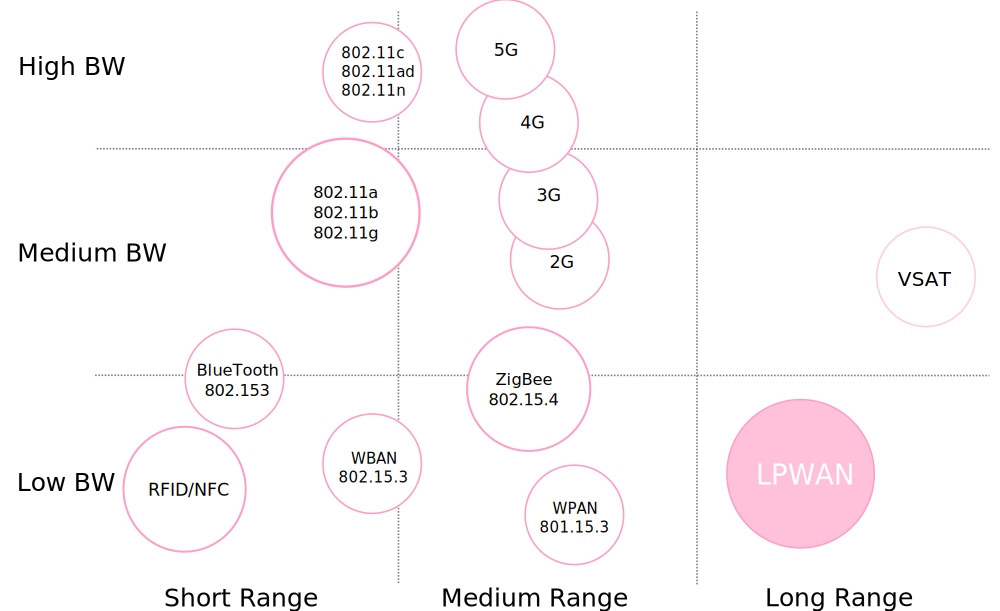
\includegraphics[width=12cm]{network-com}
    \caption{Comparazione tipologia di reti}
\end{figure}

In questo contesto, i maggiori competitor sono  NB-IoT, EC-GSM-IoT
LTE-M, SigFox e Lora. Le prime tre  sono una evoluzione delle precedenti reti
cellulari 2G,3G e 4G. Operando sulle bande di frequenza licenziate, e necessario
che ognuna di queste tecnologie sia approvata dalla 3GPP ( 3rd Generation
Partnership Project), la quale si occupa della standardizzazione dei sistemi di
telecomunicazione a livello internazionale.
All'opposto, Sigfox e Lora sono due tecnologie che operano nelle frequenze ISM
(Industrial, Scientific and Medical). Le frequenze ISM sono uno spettro radio
riservato alle applicazioni di radiocomunicazione non commerciali.

\begin{figure}[ht]
    \centering 
        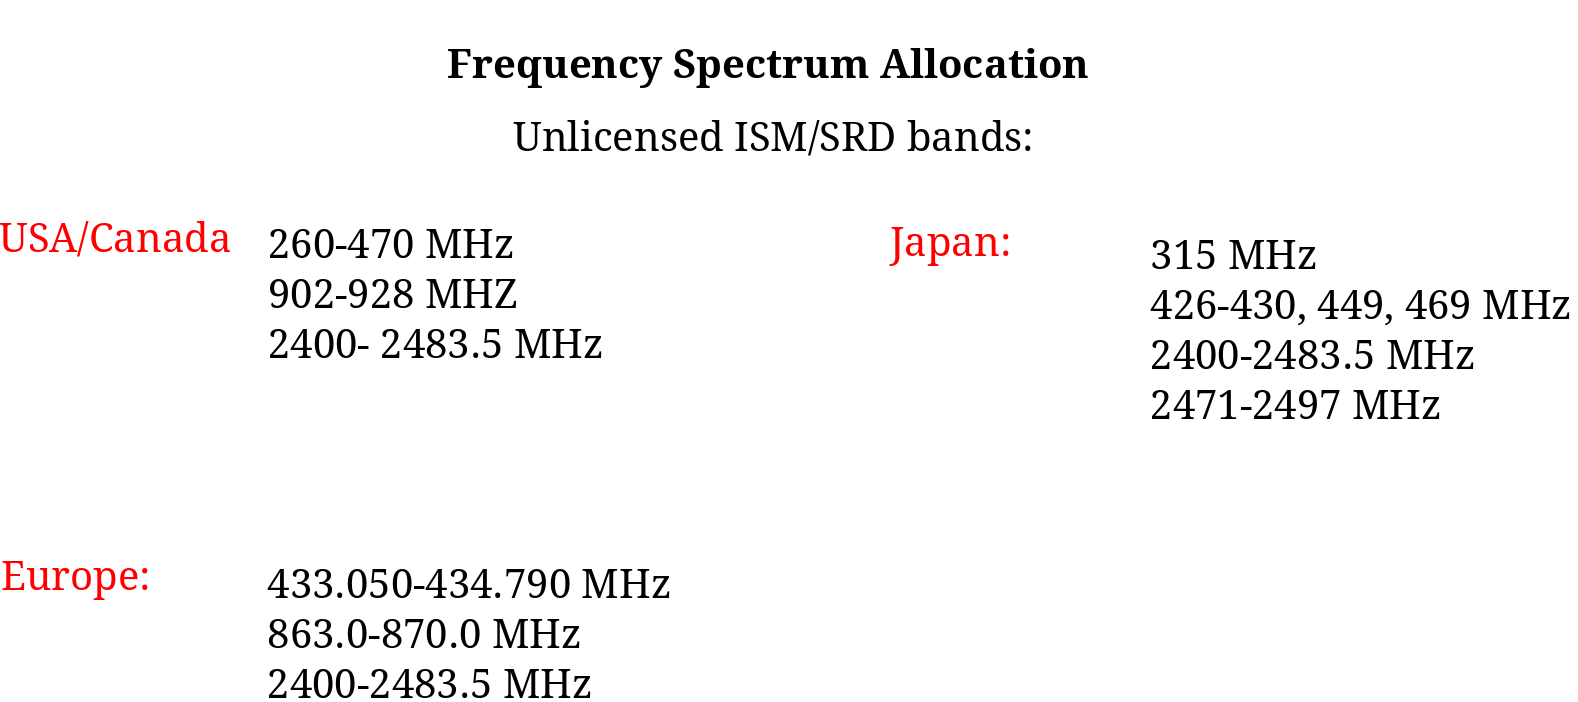
\includegraphics[width=10cm]{Orignal/freq}
    \caption{Comparazione tipologia di reti}
\end{figure}

In particolare entrambe le tecnologie operano  nella banda degli 868 [MHz]
la quale permette una potenza del segnale inviato massima pari a 14 [dbm] ed un
duty cycle inferiore al 1\%.
 
\section{NB-IoT}
Narrowband IoT (NB-IoT) o LTE Cat NB1 è uno standard certificato nella release 13 del 3GPP, la
quale riutilizza le infrastrutture già presenti, quali 2G, 3G, 4G per la rapida
realizzazione di una rete LPWA per l'IoT.
Focalizzandosi sulla durata della batteria, i moduli NB-IoT risultano avere un
costo all'unità minore del 75\% rispetto ad un normale modulo LTE.
Basato sulle frequenze licenziate, NB-IoT è in grado di
offrire tre diversi scenari di sviluppo \cite{NB-white_paper}
\begin{itemize}
\item \emph{standalone}, utilizzando qualsiasi spettro disponibile dell'
operatore.
\item \emph{guard band}, utilizzando lo spettro libero presente tra due bande
radio, per prevenire interferenze.
\item \emph{in band}, utilizzando lo stesso spettro della banda LTE.
\end{itemize}
\begin{figure}[ht]
    \centering 
        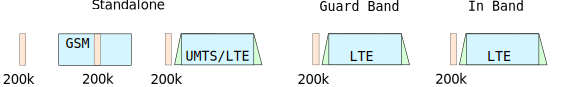
\includegraphics[width=12cm]{nb-iot}
    \caption{Modalità di funzionamento NB-IoT}
\end{figure}
L'obbiettivo che NB-IoT si prefigge è quello di mettere a disposizione una
tecnologia con una elevata copertura ed un basso data-rate. La possibilità di
riutilizzare strutture già esistenti, ed il basso costo per device , rendo
NB-IoT, una delle tecnologie che sta riscuotendo maggiore successo nel abito IoT.



\section{LTE-M}
Dalla realise 8 del 3GPP, diverse nuove tipologie di rete LTE sono disponibili.
La categoria che offre le migliori performance batteria/data-rate è la categoria
LTE Cat-M1 o LTE-M.
Questa categoria ,a differenza del NB-IoT, rispecchia lo standard LTE in pieno, 
implementando  la Frequency Division Multiplexing
(FDM) e Time Division Multiplexing (TDM). Risultando adatta per applicazioni
nelle quali è necessario l'invio di dati audio o video oppure per comunicazioni a
bassa latenza . Il data-rate raggiungibile è pari a 5Mbps in
uplink e 10 [Mbps] in downlink .  Questo tipo di connessione sarà utile
per tutte quelle applicazioni in cui è richiesta una elevata sicurezza del dato
da trasmettere, come ad esempio applicazioni di video-sorveglianza o automotive
.Questa tecnologia ,già disponibile negli Stati Uniti tramite la rete Verizon, è
in fase di roll out per molti operatori europei.

\section{EC-GSM-IoT}
EC-GSM-IoT si basa su funzionalità aggiuntive a partire da EGPRS che consentono
ad una rete GSM/EDGE di essere predisposta per fornire servizi IoT. Lo standard
è stato pensato in particolare per quei Paesi, come quelli in via di sviluppo,
dove una rete LTE non è ancora disponibile. L’occupazione spettrale di ogni
canale corrisponde a  200 kHz.  Tuttavia, al fine di dispiegare EC-GSM-IoT, si
richiede una banda utile di 2.4 MHz per permettere il frequency hopping , che,
con l’aggiunta di 2 canali di guardia di 200 kHz ciascuno agli estremi della
banda, porta l’occupazione di banda complessiva a 2.8 MHz.  La
potenza di trasmissione del Il data rate di picco raggiungibile sia in DL sia in
UL è di 491 kbps, mentre il valore mediato nominale è di 98 kbps sia in DL sia
in UL. Al fine di soddisfare i requisiti di capacità (più di 50.000 terminali in
ogni singolo settore di una cella trisettoriale). 

La figura \ref{tab:IoT_cell_comp} riassume in breve le varie caratteristiche
delle reti cellulari facenti parte della categoria LPWA
\begin{table}[h]
    \centering 
                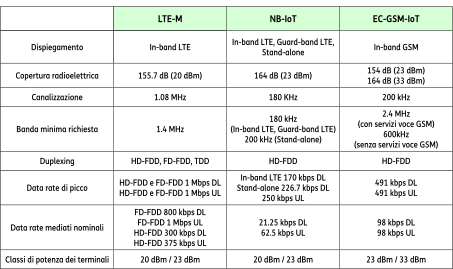
\includegraphics[width=12cm]{tim_iot}
    \caption{Comparazione reti cellulari per l'IoT}
    \label{tab:IoT_cell_comp} 
\end{table}



\section{Sigfox}
SigFox, azienda francese, sta sviluppando in partnership con altri operatori di
rete una soluzione LPWAN basata sulla sua tecnologia. Sigfox punta alla
costruzione di una rete mondiale proprietaria basata su frequenze ISM.
Correntemente SigFox è presente in Francia, Belgio, Olanda e Portogallo come
illustrato nella figura \ref{fig:Sig_covereg}.
\begin{figure}[h]
    \centering 
                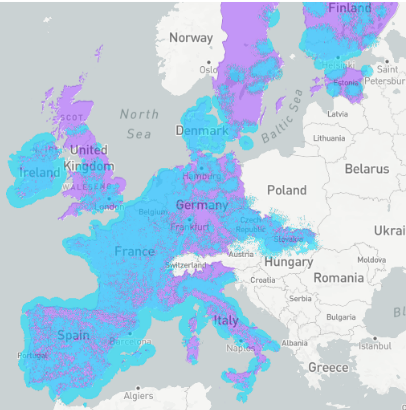
\includegraphics[width=12cm]{SigFox_covereg}
    \caption{Mappa copertura SigFox}
    \label{fig:Sig_covereg} 
\end{figure}

Gli end-devices comunicano con le varie base stations usando una modulazione (BPSK)
\emph{Binary Phase Shift Keying} con una banda di soli 100 [Hz]. 
Per via delle regolazioni vigenti nello spettro ISM, è per garantire una durata
della batteria pari ad una decina di anni, il numero massimo di messaggi
inviabili in un giorno è 140, con lunghezza del payload pari a 12 [byte] e un
throughput pari a 100 [bps]. SigFox si colloca come rete LPWAN con il minore
throughput, limitando il numero di use-case possibili. Inizialmente SigFox
supportava solo comunicazioni unidirezionali, successivamente, ha introdotto la
possibilità di avere una comunicazione bidirezionale, limitando il numero di
byte trasmissibili da gateway a devices a 4-8 bytes per giorno.

\section{LoRaWAN}
\emph{LoraWAN} è una tecnologia di modulazione wireless semi-proprietaria 
sviluppata da Semtech. Essa è composta da un layer fisico ,proprietario, che
prende il nome di \emph{Lora}\cite{LoRaCss101} , e una parte libera chiamata 
LoRaWAN\cite{LoRaWAN101} nella quale viene definito un protocollo di comunicazione, 
il quale usa LoRa come layer fisico. 
Basandosi su una tecnica di comunicazione a \emph{spread spectrum}, LoRa è in
grado di instaurare una comunicazione bidirezionale tra device e gateway.
I punti chiave dei questa tecnologia sono il grande raggio di copertura , il 
basso consumo energetico e la capacità di adattare in maniera dinamica il
data rate, il quale può variare dai 0.3 ai 50 [Kbps] a seconda dell'utilizzo. 
Come per SigFox, la tecnologia sviluppata da Semtech, si basa sulle bande ISM,
inoltre Essendo il protocollo LoRaWAN open source, si ha la possibilità di
creare delle reti pubbliche o private senza disporre di alcuna licenza, 
riducendo così il time to market di questa tecnologia.  
Progetti come \href{https://www.thethingsnetwork.org/}{The Things Network}
mirano a creare una rete LoRa ,pubblica è privata,  a livello globale.

\section{Osservazioni}
In questo mercato frammentato, non è semplice capire quale tecnologia sia adatta
a ricoprire una data applicazione. Essendo questi standard molto giovani, è
complicato comprendere le reali potenzialità di ognuna di queste soluzioni.
Quello che è possibile prevedere, sarà un incremento esponenziale di device che
stanno alla base della piramide in figura \ref{fig:pyramid}, devices i quali
potranno essere utilizzati in innumerevoli settori, non ancora esplorati dalle
tecnologie attuali, come per esempio i contatori della dell'acqua, applicazioni
per l'agricoltura di precisione e così via. 

\begin{figure}[ht]
    \centering 
                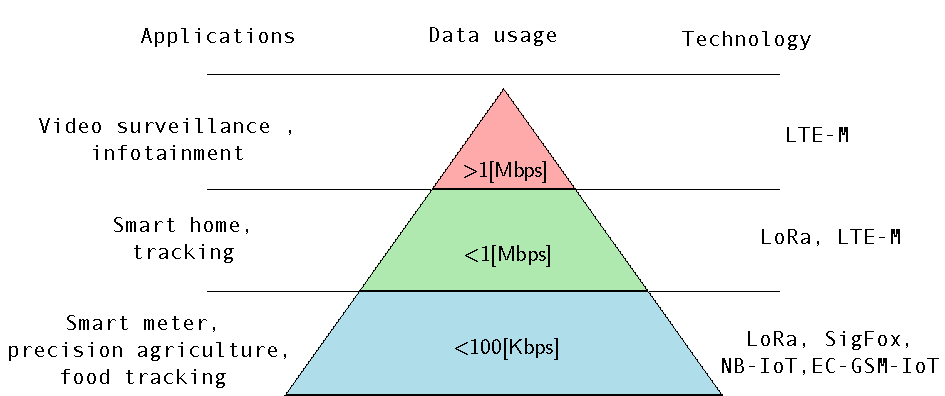
\includegraphics[width=12cm]{pyramid}
    \caption{Capacità delle reti LPWA}
    \label{fig:pyramid} 
\end{figure}

\pagebreak
Per le aziende, che si apprestano ad investire sul mondo dell'IoT, la scelta
della corretta tecnologia su cui andare a sviluppare i loro servizi non risulta
semplice, in quanto, fattori quali sicurezza, aggiornamenti software,
affidabilità devono essere ancora testati a pieno. Con la figura
\ref{fig:feature_comp} si vuole riassumere in breve i punti chiave delle
tecnologie appena trattate.

\begin{figure}[ht]
    \centering 
                \includegraphics[width=9cm]{Comparsion_no_line}
    \caption{Comparazione feature reti LPWAN}
    \label{fig:feature_comp} 
\end{figure}

Nel prossimo capitolo verrà analizzata in dettaglio la soluzione che Semtech
propone, approfondendo il layer fisico \emph{Lora} e la struttura del protocollo
LoRaWAN.


%\include{Tex_Files/Chapters/Conclusioni}


%\appendix
  
%\include{appendici}

\backmatter

\bibliographystyle{plain}
\bibliography{BiBlio/article} 

 %\printindex % se si fa l'indice analitico.

\end{document}
